\documentclass[11pt,twoside]{report}
\usepackage{preamble}
\usepackage{standalone}
\graphicspath{
	{../img/ch1/}
	{../img/ch2/}
	{../img/ch3/}
	{../img/ch4/}
	{../img/ch5/}
	{../img/ch6/}
	{../img/ch7/}
	{../img/cha1/}
	{../img/cha2/}
}

\DeclareRobustCommand{\wordcount}
{\InputIfFileExists{thesis.wordcountsum}{}{}
}

\definecolor{bristolred}{RGB}{191,47,56}


\begin{document}

\newgeometry{margin=1in}

%\maketitle
\thispagestyle{empty}
\begin{center}
  \begin{minipage}{0.8\linewidth}
    \centering
    \vspace{3cm}
    {\Large \sc University of Bristol \par}
    \vspace{2cm}
    {\Large \sc Doctoral Thesis \par}
    \vspace{1cm}
    \rule{\textwidth}{0.4pt} \par
    {\LARGE \sc \color{bristolred} 
    Observing, Analysing, Modelling, and even Changing the Behaviour of Zebrafish
    \par}
    \rule{\textwidth}{0.4pt} \par

    \vspace{2cm}
    {\large \it Author:}
    \hfill
    {\large \it Supervisors:} \\
    {\sc \large Yushi~Yang}
    \hfill {\sc \large Dr.~Thomas~Machon\par}
    \hfill {\sc \large Dr.~Chrissy~Hammond\par}
    \hfill {\sc \large Dr.~C~Patrick~Royall\par}
    \vspace{3.5cm}
   {\large \it A dissertation submitted to the University of Bristol in accordance with the requirements for award of the degree of Doctor of Philosophy in the Faculty of Science, H.\ H.\ Wills Physics Laboratory. \par}
    \vspace{1em}
    {\large March 2022 \par}
  \end{minipage}
  \mbox{}
  \vfill
  \begin{minipage}{0.8\linewidth}
    \raggedleft
    {\large 37257 Words}
  \end{minipage}
\end{center}

\pagenumbering{roman}

\cleardoublepage\documentclass[11pt,twoside]{report}
\usepackage{preamble}
\begin{document}

\cleardoublepage
\chapter*{Abstract}
\addcontentsline{toc}{chapter}{Abstract}

\cleardoublepage
\chapter*{}
\vspace*{0.2\textheight}



\noindent\emph{天涯呀~海角 ~~ 觅呀~觅知音} \\[100ex]

\noindent\emph{你的踏板车~要滑向哪里\\你在滑行里~快乐旋转着}


\cleardoublepage
\chapter*{\vspace{-1em} Acknowledgements}
\addcontentsline{toc}{chapter}{Acknowledgements}

Thank you guys!

Francesco; Erika; Paddy; John; Kathleen; Tom;
Levke; Fergus; Max; Laurent; 李静雯 (Jingwen Li);
武晓岳 (Xiaoyue Wu); 陈睿 (Rui Cheng); Katie; Wahab; 陈彦志 (Louis Chen); Jun;
My; Alessandro;
Josh; Peter;
BCFN; Fish Facility; Zebrafish;
王敏 (Min Wang); 杨冬 (Dong Yang);


\cleardoublepage
\chapter*{Author's declaration}
\addcontentsline{toc}{chapter}{Author's declaration}

I declare that the work in this dissertation was carried out in accordance with the requirements of the University's Regulations and Code of Practice for Research Degree Programmes and that it has not been submitted for any other academic award.
Except where indicated by specific reference in the text, the work is the candidate's own work.
Work done in collaboration with, or with the assistance of, others, is indicated as such. Any views expressed in the dissertation are those of the author.

\vspace{1cm}
\vspace{-3pt}

\hspace{2.5cm} {\huge\emph{杨雨诗}} \hspace{5.5cm} 30/01/22 \vspace{-\baselineskip} \vspace{3pt} \\
SIGNED: .............................................................
\qquad
DATE: ..........................

\vspace{1cm}

\section*{Contributions:}

\cite{yang2021pcb}\; \fullcite{yang2021pcb}. \\

\end{document}

\cleardoublepage

{
	\hypersetup{linkcolor=black}
	\tableofcontents

	\cleardoublepage
	\listoffigures
	\addcontentsline{toc}{chapter}{List of figures}
	
	\cleardoublepage\listoftables
	\addcontentsline{toc}{chapter}{List of tables}
	
	\listofalgorithms
	\addtocontents{loa}{\def\string\figurename{Algorithm}}

}

\printnoidxglossary[
	type=acronym, style=list,
	title={List of Abbreviations}
]

\newpage

\printnoidxglossary[
	type=symbols, style=mylong3colheader, title={List of Symbols}
]

\cleardoublepage
\restoregeometry

\pagenumbering{arabic}

\pagenumbering{arabic}
\setcounter{page}{1}%

\documentclass[11pt,twoside]{report}
\usepackage{preamble}
\graphicspath{{../img/ch1/}}
\setcounter{chapter}{0}


\begin{document}
\chapter{Introduction}

This thesis will discuss the behaviour of zebrafish from the perspective of soft--matter physicists. It is expected that we can get some general insights about animals, by analysing their trajectories. Operationally, it means to tabulate the location of different individuals at different time points, and then analyse the shape of the line segments connecting all these points. One can imagine that most people's trajectory will be centred around workspace and home, connected by their commute routes. And a large group of people sharing similar trajectories might indicate the presence of a parade.

By doing so, we discarded all the details of each individual, and this is exactly the point. The physicists propose \emph{coarse--grained} models that deliberately ignore the details, in order to focus on the phenomena on larger scales. For instance, we know the different types of liquid flow differently, with different viscosities. The concept of viscosity let us to grasp the essence of liquid, rather than the detailed information of the constituting molecules. Formally, we say that we ignore the microscopic detail (the shape and chemistry of the molecules), and focus on the macroscopic behaviour (the viscosity).

However, there is one fundamental difference between the living animal and moving atoms/molecules. In daily life, most atomic/molecular systems were in \emph{equilibrium}, being in a state that ``nothing happens''. By definition, the equilibrium system will enter and leave any microscopic state at the same rate, maintaining the same macroscopic behaviour constantly. And this situation is very different when we think about animals, where the individuals were ageing, the territories were changing, and the gross domestic productivity (GDP) increasing.


% Separation of time scale
Luckily, physicists have a powerful tool to attack the problem. The tool is \emph{time--scale separation}, which treat fast phenomena differently from their slow counterparts \cite{gunawardena2014}.

% Separation of time scale

 The idea comes from a subbranch of soft--matter physics, named \emph{active matter}, which focuses on the self--propelling non--equilibrium systems\marginfootnote{Not all non--equilibrium systems are called active matter. An example is the driven system, where the system is exposed to applied strain.}.
Here comes the essence of idea. Ignoring some biological details, we can treat individual animals as moving agents with simple interaction rules. And this assumption is backed up by computer simulations of idealised models, as these simulations reproduced natural collective behaviour of animals.

\section{Thesis Structure}

The ideas of active matter and the collective behaviour of animals will be introduced in chapter \ref{chapter:collective_behaviour}.


Analysing the behaviour of fish turns out to be a technical and complicated task, if one wants to study them in a three dimensional environment. Consequently, building the system that records the 3D movements of fish became a big part of this study, and I will introduce the technology in two steps. Firstly the easier setup to capture the 2D movements of the zebrafish will be discussed in chapter \ref{chapter:fish_2d}, along with necessary data processing methods. The relevant experimental results will also be presented in this chapter. Then we shall move on to setting up the 3D tracking system, discussed in detail in chapter \ref{chapter:fish_3d}. Specifically, the ideas in the multiple view geometry will be introduced, which enables the 3D reconstruction of the fish locations. The experimental findings of 3D tracking will also be discussed in chapter \ref{chapter:fish_3d}.

A further understanding of the fish can be achieved by modelling their behaviour. And we know the model is good if the behaviour of the model matches the experimental results. Different models will be introduced and discussed in chapter \ref{chapter:fish_model}. The experimental results from chapter \ref{chapter:fish_2d} and \ref{chapter:fish_3d} will be compared with different models.

Finally, we will advance to a more biological topic and discuss the behaviour of zebrafish after genetic modification. In chapter \ref{chapter:fish_mutation}, the collective behaviour of the mutant fish will be reported and compared against the normal, wildtype zebrafish. The insight into the mutation fish is only available through the behavioural experiments. And the result in this chapter is the evidence, that active--matter physics can offer new biological knowledge about animals. In other words, this thesis is \emph{useful}.

\end{document}
\documentclass[11pt,twoside]{report}
\usepackage{preamble}
\graphicspath{{../img/ch2/}}
\setcounter{chapter}{1}


\begin{document}


\chapter{The Collective Behaviours out of Equilibrium}

\epigraph{We declare that the splendour of the world has been enriched by a new beauty: the beauty of speed.}{F. T. Marinetti, \emph{Manifesto of Futurism}, (1909)}

This chapter would introduce the readers the background of non-equilibrium collective behaviours. Mainly this chapter will be about the collective behaviours of \emph{animals}.

\section{Facets of Collective Behaviours}

\subsection{Understanding Animals}

\subsection{Controlling Robots}

\subsection{Active Matter Physics}


\section{Observations and Experiments}

Experimentalists observed different types of collective behaviours. In this section I will categories these phenomena according to the spatial dimensions. 

\subsection{Collective Behaviours in 0D}

The collective behaviours of animals can happen without space. One example is the sound of fogs.

\subsection{Collective Behaviours in 1D}

\subsection{Collective Behaviours in 2D}

The movement of fish had interested researchers, and people had been embedding the idea from condensed--mater physics in the fish study since 1978. \cite{}

\subsection{Collective Behaviours in 3D}

\subsection{Collective Behaviours other Dimensions}

\section{Modelling The collective Behaviours}

\subsection{The Vicsek Model}

\subsection{Vectorial Network Model}

A well studied model is the 2D Vectorial Network Model (VNM). Sharing the same velocity updating rule with the Vicsek model, the VNM used a graph to determine the neighbours between particles, instead of determining the neighbours based on the spatial relationships. 

The disordered states are composed of purely randomised vectors. The order parameter, noted as the polarisation $\Phi$, is constantly 0.

\citeauthor{aldana2003} analysed the model in detail, and claimed the continues phase transition in VNM can be described by equation \cite{aldana2003},

\begin{equation}
	\Phi=\left\{\begin{array}{ll}{\left[C\left(\eta_{c}-\eta\right)\right]^{1 / 2}} & \text { for } 0<\eta_{c}-\eta \ll 1 \\ 0 & \text { for } \eta>\eta_{c}\end{array}\right.	
\end{equation}

\noindent where $\Phi$ is the polarisation order parameter, $\eta$ is the noise level, and $\eta_c$ is the critical noise value. In addition, the relationship between the polarisation ($\Phi$) and $\eta$, near the critical point, is approximated by

\begin{equation}
\Phi \approx \sqrt{
	\frac{2(\sin \eta-2 \eta)}{(K-2) \sin \eta-(K-3) \eta}\left(1-\frac{\eta}{\sqrt{\pi K} \sin (\eta / 2)}\right)
},
\end{equation}

\noindent where $K$ is the number of neighbours of the particles. The result matches the numerical results. This analytical expression covered the ``critical'' region of the model, and can not be extrapolated to the ordered states.

Years after \citeauthor{aldana2003}'s work, \citeauthor{porfiri2014} derived the expression for the ordered states VNM, which writes as \cite{porfiri2014}

\begin{equation}
\Phi \approx 1-\eta^{2} \frac{\pi^{2}}{6} \frac{K(N-1)}{N(K-1)+1},
\end{equation}

\noindent where $N$ is the number of particles.

\subsection{The Inertial Spin Model}

The inertial spin model is another important variant of the Vicsek model, where the dynamic of the system is given by the following Hamiltonian.



\subsection{The Active Brownian Models}

\subsection{Other Agent Based Models}


\end{document}

\documentclass[11pt,twoside]{report}
\usepackage{preamble}
\graphicspath{{../img/ch3/}}
\setcounter{chapter}{2}



\begin{document}

\chapter{Observing Zebrafish in 2D}
\label{chapter:fish_2d}




In this chapter we will focus on the methodology to observe zebrafish, swimming in a quasi two dimensional environment. The system was chosen for technical conveniences, as the 2D movement of fish can be captured by a digital camera easily. In comparison, recording the 3D movement of fish is a harder task, which will be discussed in chapter~\ref{chapter:fish_3d}. %and appendix~\ref{chapter:multi_view}.


\section{Introduction}


The majority of the studies on the collective behaviour of fish were performed in a quasi-2D environment, where the fish were confined in a shallow water tank \cite{miller2007, strandburg-peshkin2013, heras2019, sridhar2021}. The collective motion of the fish can be captured by digital cameras and process by image processing algorithms, generating the trajectories for all fish individuals.
%\marginfootnote{The zebrafish were usually recorded as grayscale videos, in contract to the coloured videos taken by conventional cameras. This is because the zebrafish are not colourful. Therefore, the different colour channels (red, green, blue) are often not very helpful for identifying the fish individuals in the video.}

The crucial step in this tracking process, is to correctly locate the fish, and identify their identities. A considerable amount of softwares have been designed to tackle the problem. For instance, \citeauthor{perez-escudero2014} published an algorithm that is capable of determining the identity of the fish from its image, and using the information to obtain correct trajectories \cite{perez-escudero2014}.
The key observation from \citeauthor{perez-escudero2014}, is that the joint probability distribution of pixel distance and pixel intensity of a fish is unique. Five years later in 2019, the same group published an update method, that utilised an artificial neural network to identify the individual fish \cite{romero-ferrero2019}.
Unlike most machine learning solutions to computer vision problems, the algorithm from \citeauthor{romero-ferrero2019} requires no human label, thanks to a very carefully constructed preprocess pipeline, which makes it stands out as the state of art method in the year of 2022 \cite{walter2021}.


In addition to the ideas and algorithms, the realistic development and deploy of an animal tracking software requires a lot of engineering work. For instance, it is important to have a suitable programming language to maximise the performance of the algorithm. An accessible graphical user interface (\gls{GUI}) and application programming interface (\gls{API}) are also crucial. In addition, the software should be easy to install on a new machine. Practically, large research groups will develop a versatile research software, like those from \citeauthor{walter2021} \cite{walter2021}.


In this chapter, We will present a new 2D tracking method, whose results are suitable for the calculation of 3D locations of the fish. The key feature of our algorithm is the ability to locate fish without relying on their morphological details (see Fig.~\ref{fig:fish-detail} for examples).
Our new method is necessary, because the fish can swim closer or further to the camera in the 3D experiment, casting different shapes on the camera.
Therefore, the identity of the fish can not be uniquely determined from their shapes in the image, causing the identity-based approach (\cite{perez-escudero2014, romero-ferrero2019, walter2021}) to have reduced validity. The problem is termed \emph{no-detail tracking}, as the details (the size, darkness, and shape) of a fish in the image is not a reliable source for its identification.

\marginpar{
\centering
\includegraphics[width=\marginparwidth]{fish-detail}
\captionof{figure}[The morphological detail of a fish]{
	Top: a picture of zebrafish with various details. Bottom: a picture of two zebrafish with no detail.
}
\label{fig:fish-detail}
}

In the methods section, the ideas needed to carry out no-detail tracking will be discussed. The result of 2D swimming experiment, analysed by our method, will be presented in the results section. The 2D coordinates of zebrafish revealed two essential features. Firstly the spatial distribution of the fish was inhomogeneous. The effective pairwise interaction of the fish seemed attractive, and the attraction appear to decrease with the number of individuals in a group.

\section{Methods}

%Observing the fish in the lab includes the construction of the hardware, and the development of the software. Both of them will be covered in the method section. The 2D tracking code will be reused in chapter~\ref{chapter:fish_3d} as the basis for 3D tracking. 

\subsection{Fish and Apprautus}
\label{section:apprautus_2d}

The adult zebrafish, whose age is over one year old, were used to carry out the experiment. Most experiments in this section was carried out in the fish facility in Bristol, while some experiments were performed in room G59 in the HH Physics Laboratory in Bristol. The fish were fed three times a day, with natural day to night circles. The fish were hosted in their living tank before the experiments, with a density of 5 fish per litre of water. The water was filtered constantly, with a pH value close to 7 and the temperature close or above 25 °C.

Before each experiment, the fish were transferred from their living tank to the experimental environment, which will be referred to as the {\ot}. During the transfer, the fish were placed inside a temporary container, and then released into the {\ot}.
To make the fish stay in a quasi-2D environment, a flat plate was placed in a bowl-shaped tank, creating a shallow water environment (Fig.~\ref{fig:fish_apprautus_2d}). The shape of the bowl is especially chosen for a 3D tracking task, which will be introduced in chapter \ref{chapter:fish_3d}.



\begin{SCfigure}[][!ht]
  \includegraphics[width=\linewidth]{apprautus-2d}
  \caption[Two dimensional fish tracking apprautus]{\label{fig:fish_apprautus_2d}
  The apprautus to track the movement fish in a quasi-2D environment. The camera is placed above the fish to capture the top view. A computer controls the recording process as well as the illumination.
  }
\end{SCfigure}


\subsection{Metric Rectification}
\label{section:metric_rectify}


To record the video of the fish, a camera (Basler AC2040um) was fixed on top of the tank, as illustrated in Fig.~\ref{fig:fish_apprautus_2d}. The image size produced by our camera is 2056 pixels $\times$ 1540 pixels, at a frequency of 15 frames per second.
We mounted a 6 mm fixed focal length lens (C Series, Edmund Optics) on the camera, which yields a wide view, allowing us to place the camera closer to the fish group. The typical distance between the camera and the fish group is around 2 meters. With such setup, the fish (body length $\sim$ 30 mm) appear as black rods in the videos, as shown in Fig.~\ref{fig:metric-rectify}.


The image and videos obtained from the camera have three limitations, preventing it from being an accurate measurement tool.
The first issue is the distortion of images caused by the camera lens.
In addition, the cameras should be orientated exactly perpendicular to the water surface, so that the captured images were from the top view. Such accurate orientation is difficult to achieve without especially designed camera holders.
Finally, we also need to convert the unit of the image (pixels) to real life units (e.g. meters).
It is worth mentioning that these issues were more or less ignored in conventional 2D animal tracking tasks \cite{panadeiro2021}, and the present method is novel in the context of animal tracking.\marginfootnote{
Addressing these issues is ``less novel'' in the computer vision community focusing on the 3D reconstruction. It is impossible to retrieve 3D information correctly without understanding all the details about computers and photos.
}

To solve the problems, we need to \emph{calibrate} the camera, so that we know the distortion of the camera lens, the orientation of the camera, as well as the scale of objects in the images. To carry out the calibration, a chessboard (the calibration board) was placed on the surface of the water. And the image of the calibration board will offer enough information to tackle the aforementioned issues. 

The distortion can be recovered with standard camera calibration methods\marginfootnote{
The functions from the ``opencv'' library were used for the calibrations.
}
from the computer vision community \cite{ma2005, hartley2003}. The distortion is described with the following model,

$$
\begin{aligned}
x_{\text {distorted }} &= x\left(1+k_{1} r^{2}+k_{2} r^{4}+k_{3} r^{6}\right) \\
y_{\text {distorted }} &= y\left(1+k_{1} r^{2}+k_{2} r^{4}+k_{3} r^{6}\right)
\end{aligned}
$$

\noindent where $r$ is the radius of the pixels in the image with respect to the optical centre. And $k_i$ values are the distortion coefficients, which will be used to recover the undistorted image.


The imperfect orientation can be fixed by the knowledge of the camera as well. Briefly, the same 2D plane in the 3D space, will form different projections with different cameras. 
These different 2D projections are related to each other by a projective transformation.
Likewise, the same 2D plane for the fish in the imperfectly orientated camera is also related to its counterpart from a perfectly orientated camera.
Such a relation is termed as \emph{homography}
%\marginfootnote{Further description of the projective transformation, as well as the calculation of $\mathbf{H}$ is included in the appendix~\ref{chapter:multi_view}.}
, and can be represented by a matrix
$\mathbf{H} \in \mathbb{R}^{3 \times 3}$. This matrix can be calculated easily with the knowledge of the camera, following the method from \citeauthor{hartley2003} \cite{hartley2003}.
The homography allows us to transform the image from the imperfectly orientated camera, to a virtual image captured from a perfectly orientated camera. The transformed image is called the \emph{rectified image}.
From the rectified image, the scale can be recovered easily as we know the physical size of the calibration board. We call the rectified image with a known scale the \emph{metrically rectified image}.


Figure~\ref{fig:metric-rectify} shows an example of the metric rectification. Comparing the outline of boundary with/without distortion removed, it is clear that the raw image from the camera were distorted by the lens. The camera in the experiment were not perfectly perpendicular to the water surface, therefore the outline of the tank boundary appears to be an ellipse, because of the perspective transformation (\gls{homo}). The ellipse were reverted back to a circle (right subfigure, Fig.~\ref{fig:metric-rectify}) after the rectification process.

\begin{SCfigure}
  \includegraphics[width=\linewidth]{image-calib-2d.png}
  \caption[Metrical rectification of an image.]{
  	The process of metrical rectification. Left: the original image. Middle: the image where camera distortion being removed. Right: the metrically rectified image. The circular outline of the 2D boundary were outlined and overlaid, to stress the change of the image in different steps. The inserts in the figures correspond to the calibration pattern in each process.
  }
  \label{fig:metric-rectify}
\end{SCfigure}


Notably, the image rectification only ``works'' for the plane, where the calibration chessboard lies. For the fish data, the rectification is only accurate for the fish exactly swimming on the water-air interface. In other works, there will be tiny errors for the fish locations, when they swim inside the water. Such inaccuracy is fundamental for 2D fish tracking, since the fish is swimming a 3D space. To eliminate such error, we can carry out real 3D measurements, which will be introduced in chapter~\ref{chapter:fish_3d}.


\subsection{Image Processing}
\label{section:image_process}


The metrically rectified images of the fish contain the information about their behaviour.
To get useful information out of the image, we still need to perform image processing, to extract the coordinates of the fish from the images.

In a normal image, the fish appear as a dark spot (see Fig.~\ref{fig:metric-rectify} and Fig.~\ref{fig:2d_process} for instances).
Ideally, we want to work with images containing a collection of delta functions (see middle subplot of Fig.~\ref{fig:locate-cnn} for instance), where the pixel intensities in the centres of each individual fish is maximised, and the pixel intensities are zero everywhere else. Extracting the coordinates of fish from such image, will therefore be a trivial task, as we only need to find the pixels with non-zero values. Even though it is possible to construct such transformation directly with machine learning based approaches \cite{newby2018}, it is still not an easy task, without large amount of human labelled training data. Therefore, we restrict our goal for the image processing process to be the removal of the static background. As a result, the processed image should only contain the fish.

Traditional image processing methods, such as thresholding, blurring, and morphological operations, were used in this project to perform the background removal task.
As a result, we get a \emph{foreground video} where each fish has high pixel intensity values, and the background intensity values are zero. Figure \ref{fig:2d_process} illustrates the result of the transformation. One frame of the recorded video was shown in the left subfigure, while the same frame from the foreground video was shown in the right subfigure.


\begin{SCfigure}
  \includegraphics[width=\linewidth]{image-process}
  \caption[Two dimensional image processing.]{
  The screenshot of the video at time point $t$, and its corresponding foreground image.
  }
  \label{fig:2d_process}
\end{SCfigure}


The foreground videos of the fish are obtained after two  steps, the removal of the background and the removal of the noises. 
The background is defined as the temporal average of the image, since the fish are constantly moving while rest of the scene is static. In order to tackle the varying illumination conditions\marginfootnote{
The brightness of the environment might change in the field observation, where the sunlight might be temporally covered by the cloud. In the laboratory, the sunlight will also change the overall brightness indoors.
},
we can take a running average of a time--window, instead of calculating the overall average. The pixel intensity of the background (\gls{bijt}) at time \gls{t}, of pixel $(i, j)$, can be written as

\begin{equation}
	B_{ij}(t) = \frac{1}{T_w} \sum_{\tau=t}^{t+T}{I_{ij}(\tau)}
\label{eqBG}
\end{equation}

\noindent where \gls{iijt} is the pixel intensity of the video at time \gls{t} in position $(i, j)$, and $T_w$ is the duration of the window, usually taken as 40 seconds. The difference between the background video and original video yields a foreground video (\gls{fijt}), written as

\begin{equation}
	F_{ij}(t) = B_{ij}(t) - I_{ij}
\label{eqFG}
\end{equation}

\noindent and the order of the subtraction ensures the fish, originally appear darker in the video, to be represented by brighter pixels in the foreground video. The subtraction result can be very noisy. To remove the noise, the gaussian filter was applied to the foreground image. Then, the combination of the Ōtsu threshold and local Gaussian threshold was applied to the image, to separate the pixels belonging to the fish and other pixels.
The Ōtsu threshold is a single value that split the image into two groups, where the inter--group variance was minimised. The local Gaussian threshold, on the other hand, gives a collection of different values for different pixels, featuring the locally bright pixels as foreground. Finally, the morphological operation ``binary opening'' was applied to the image, to remove any possible remaining noise. The results shown in Fig.~\ref{fig:2d_process} was obtained with this method.

Our method requires 3 parameters, including the standard deviation (\gls{sigblur}) of the  Gaussian kernel of the blurring process, the length scale for the local threshold (\gls{llt}), and the length scale of the binary open operation (\gls{lbo}). In the different experiments, the images were similar, therefore the same set of parameters ($\sigma_\mathrm{blur}=2, l_\mathrm{local}=3, l_\mathrm{open}=3$) was applied, and works well for most videos.



\subsection{Extracting Features from the Image}
\label{section:feature}



From the processed video, we need to extract the features\marginfootnote{
We explained the term ``features'' by the end of the section.
} in each frame that correspond to the fish. In order to tackle the problem, we employed a method that not only captured the positions, but also the information of the fish orientations and body shapes. The basic idea is to calculate the cross--correlation between the image ($F_{ij}$) and a templated fish shape (\gls{tij}), as the local maxima in the result would indicate the presence of a fish, because cross--correlation is a measure of similarity between signals.


For a fixed 2D fish template (\gls{tij}), we can rotate it so that it contains $o$ different orientations. Calculating the cross-correlation of all the rotated templates, we can effectively get $o$ different results, and they can be concatenated into a 3D tensor, written as \gls{cijo}. One can think of the tensor $C_{ijo}$ as a 3D volumetric image. A local maximum in $C_{ijo}$, with coordinate $(i_m, j_m, o_m)$, indicates the presence of a fish at location $(i_m, j_m)$, with orientation $o_m$.


In addition, we are free to choose different templates for the fish shape, to capture the different postures. The choice for the template will be discussed in section~\ref{section:template}. If $s$ different shapes were selected as templates, all of which were rotated into $o$ different orientations, then there will be $s \times o$ different templates. The cross-correlation of these templates with the image would yield a 4D tensor that can be shaped into \gls{cijos}, noted as the \emph{feature tensor}. A local maximum of the feature tensor, with coordinate $(i_m, j_m, o_m, s_m)$, represents a fish located at $(i_m, j_m)$, whose shape is like the $s_m$th template, with orientation $o_m$. All the local maxima, {$\{(i_m^i, j_m^i, o_m^i, s_m^i)\}$}, captured the locations, orientations and shapes of all the fish in the image.

\begin{SCfigure}
  \includegraphics[width=\linewidth,outer]{features}
  \caption[The correct label of overlapping fish.]{
  The locations and orientations, $\{(i_m, j_m, o_m)\}$, of different fish. The locations are rendered as circles, while the orientations were rendered as short line segments.
  The features were calculated from the feature tensor ($C_{ijo}$).
  Top: the movement of 4 fish in 6 successive frames labelled with the detected features. An error where one fish was mistakenly labelled as two fish happened in the 6th frame.
  Bottom: the movement of many fish labelled with the detected features.
  }
  \label{fig:fish_features}
\end{SCfigure}

In summary, the cross--correlation between the image and the many templates yields a 4D feature tensor, whose local maxima give us the locations, orientations, and shapes of different fish. This approach is especially helpful for the dense system, where the fish constantly overlap with each other. In such dense scenario, the overlapping fish will be separated into different regions in the shape--rotation dimension in the feature tensor. For example, the overlapped fish pair in Fig.~\ref{fig:fish_features} was correctly labelled, by calculating the local maxima in the 4D tensor.


There is a fundamental flaw of our algorithm, where a big fish might be mistakenly labelled as two small fish. One example of such error was presented in Fig~\ref{fig:fish_features} (top row, t=6).
This is partially due to the loss of morphological details of the fish, as the cameras were placed relatively far from the fish, in order to capture larger groups.
Without the details, it can also be hard for a human being to tell, whether a dark blob is a big fish or it belongs to two smaller fish. Realistically, some of the errors produced by our algorithm can be easily distinguished by human beings. Some post processing methods of the features, based on the geometry of the fish, might be useful to further refine our algorithm. The ultimate goal is to make the feature detection algorithm being compatible with human observations.


\begin{tcolorbox}[
title={Why are features called features, not positions?},
enlarge bottom by=0.5em,
enlarge top by=0.5em,
]
In the computer vision community, people call the locations of objects ``features''. This term is rooted in the 3D reconstruction problem, which will be discussed in the chapter~\ref{chapter:fish_3d}. Briefly, the 3D information can not be recovered from the background, like a purely white wall. Instead, some ``features'' with intensity gradients are required \cite{ma2005}. Alternative names would be ``positions'' or ``locations''. However, we are interested in a ``feature'' of the photo, rather than a (physical) location of a fish.
\end{tcolorbox}

\subsection{Finding Templates for the Features}
\label{section:template}


To calculate the feature tensor $C_{ijos}$, it is important to use suitable templates for the fish. The templates should represent characteristic fish shapes.
%The unsupervised machine learning methods from the computer vision community are suitable in this situation .
The following operations were carried out to find suitable templates.

\begin{enumerate}
	\item Segment the individual fish and align the segmented images.
	\item Project all the segmented images to a space with reduced dimension.
	\item Find clusters for the data points in the reduced space, and the average of each cluster to be the template.
\end{enumerate}

The individual fish, defined as connected bright pixels, were segmented from the foreground video ($F_{ij}(t)$).
The orientation of the segmented fish were determined by the principle component analysis (\gls{PCA}) \cite{goodfellow2016}. 
These segmentations were then reoriented, so that its first principle axis align with the $x$ axis. The reoriented individual fish were then zero-padded to have the same shape, noted as $\mathbf{S} \in \mathbb{R}^{s \times s}$ where $s$ is the size of the padded images.
Examples of the segmented and aligned images are illustrated in Fig.~\ref{fig:fish_segment}. These images were collected over 1000 different frames, in a video of 4 swimming fish. A total of 3070 individual shapes were collected.

\begin{SCfigure}
  \includegraphics[width=\linewidth]{shapes}
  \caption[Examples of segmented individual fish]{
  Top: the selected individual fish segmented from the images taken by the camera.
  Bottom: the fish shapes reconstructed from a low dimensional feature space $\mathbf{X}_\mathrm{red}$.
  }
  \label{fig:fish_segment}
\end{SCfigure}

The collection of segmented fish is a very large dataset.
For example, if we use a small image of size $50 \times 50$ pixels, to stored each fish, then each fish corresponds to a point in a 2500 dimensional space.
The dimension of such images can be drastically reduced by PCA \cite{solem2012book, geron2019}. Operationally, all of the $m$ images of individual fish were flattened
($\mathbb{R}^{s \times s} \rightarrow \mathbb{R}^{s^2}$),
and concatenated into a matrix ($\mathbf{X} \in \mathbb{R}^{m \times s^2}$).% For the dataset presented in Fig.~\ref{fig:fish_segment}, $m=3070$.
The singular value decomposition (\gls{SVD}) is then performed on the dataset $\mathbf{X}$, following

$$
\mathbf{X} = \mathbf{U} \Sigma \mathbf{V}^T,
$$

\noindent where the matrices $\mathbf{U}$ and $\mathbf{V}$ contains all the left and right singular vectors, and the matrix $\Sigma$ contains all the singular values. The images ($\mathbf{X}$) were then project on the first $k$ axes ordered by their corresponding singular values. Effectively, the dimension of the matrix $\mathbf{X}$ were reduced from $m \times s^2$ to $m \times k$, forming a new matrix $\mathbf{X}_\text{red} \in \mathbb{R}^{m \times k}$. Each row in $\mathbf{X}_\text{red}$ described one fish.



Figure~\ref{fig:fish_pca} shows the average fish shape as well as the projection of all the segmented fish ($\mathbf{X}$) on the first two principle axes. The first principle axis (the $x$ axis of Fig.~\ref{fig:fish_pca}) roughly captured the scale of the fish, and the second principle axis (the $y$ axis of Fig.~\ref{fig:fish_pca}) captures the information about the bending of the fish. 
The overall distribution of those projected data can be understood by the fact that the same fish can have different distances and orientations, relative to the camera, so that their shapes will appear different.
The distribution of Fig.~\ref{fig:fish_pca} is symmetric in the $y$ direction, which indicates the absence of chirality for the bending of fish. That is to say, the fish do not prefer bending to the left, or the right.

With all the segmented fish being projected to low dimensional space, we can use the \emph{k-means cluster} algorithm to find representative cliques of the fish shapes.
Briefly, different data points (different fish images in Fig.~\ref{fig:fish_segment}) will be assigned to different clusters. And the variance of points in the same cluster will be minimised, while the variance of points from different clusters will be maximised.

Each cluster corresponds to similar fish images with similar shapes. The average shape of different clusters were used as the template. The different scatters in Fig.~\ref{fig:fish_pca} shows the different clusters, and their corresponding average shapers were inserted. Here, the images ($\mathbf{X}$) were projected to a 2 dimensional space ($k = 2, \mathbf{X}_\text{red} \in \mathbb{R}^{3070 \times 2}$). And the overall 3070 points were separated into 7 different clusters. And the average shape of different clusters (the inserted subplots in Fig.~\ref{fig:fish_pca}) can be used as the templates to calculate the 4D tensor for tracking.



\begin{SCfigure}
  \includegraphics[width=\linewidth]{fish-pca-proj}
  \caption[PCA analysis of the fish shape]{
  A collection of 2170 different fish shapes, projected onto the first two principle component axes. The data points were clustered using the K-means algorithm, into six different clusters, indicated by different marker styles. The average shape of each cluster were plotted in the inserted axes.
  }
  \label{fig:fish_pca}
\end{SCfigure}


The number of clusters and the dimension of the reduced space ($k$) are free parameters, whose optimal values were hard to determine. Practically, I always set $k=5$, and separate the points into 8 different clusters, which yields good\marginfootnote{
If the 2D features are not good, the corresponding 3D reconstruction (chapter~\ref{chapter:fish_3d}) will fail.
} results for 2D tracking. The dimensional reduction method (PCA) and the clustering algorithm (K-means) can be changed to other tools with similar effects. For instance, it is possible to use non-linear dimensional reduction method such as isomap, and a gaussian mixture model to obtain different clusters.

The mapping from the image to the large 4D tensor, $I_{ij} \rightarrow C_{ijos}$ requires a large amount of calculation. The feature tensor is normally sparse, since only a few pixels in the image contain the centre of the fish. The calculation can be faster if such sparsity were to be exploited.
Practically, we can only calculate ``promising'' pixels, where fish is likely to appear. These pixels correspond to the local intensity maxima in the foreground image $F_{ij}$. Such reduction of calculation improved the calculation speed significantly.


\subsection{Convolutional Neural Network}
\label{section:cnn}



There are two steps in the image processing that can be improved in the image processing pipeline. The first one is the removal of background. In my current method, I calculated a rolling average of the entire video. The window size of the averaging operation is set by the user, which is very difficult to optimise because the video processing typically takes hours to finish. Practically, a rule-of-thumb number (600 frames) was applied. However, the fish in the video are very distinct from their background, and it is an easy task for people to spot the fish in a static image. This suggests a static image contains enough information to distinguish the foreground (fish) and background (tank). 

The convolutional neural network (\gls{CNN}) is very suitable for carrying out both tasks at the same time, with far better efficiency. The overall data process introduced from section~\ref{section:image_process} to section~\ref{section:template}, is essentially a transformation from the image ($I_{ij}$) to a tensor ($C_{ijos}$). In addition, the information about the kernel is unnecessary\marginfootnote{
The shapes might be informative for people studying the postures of the swimming fish. But we will ignore the shapes in this thesis as we are interested in the \emph{collective motion} of the fish.
} in most cases, as we often only care about the orientation and location of the fish, rather than its shape. Hence, we need a model with the capacity to carryout the following transformations depending on our desired results:

$$
\begin{aligned}
I_{ij} &\rightarrow C_{ijos} 
&\textrm{location, orientation, and shape} \\[1ex]
I_{ij} &\rightarrow C_{ijo}\;(= \max_{s}{C_{ijos}})
&\textrm{location, and orientation} \\
I_{ij} &\rightarrow C_{ij}\;(= \max_{o}{C_{ijo}})
& \textrm{location} \\
\end{aligned}
$$

\noindent And we can generate a big dataset containing images ($I_{ij}$) and their corresponding feature tensors ($C_{ijos}$), and make a CNN to learn the underlying rules for the transformation ($I_{ij} \rightarrow C_{ijos}$). If we need less information from the result, the targeted $C$ can be contracted, by taking the maximum value along the dimension of the unnecessary information.

\begin{SCfigure}
  \includegraphics[width=\linewidth]{locate-cnn}
  \caption[The feature tensor calculated with convolutional neural network]{
	The tracking result of a convolutional neural network (CNN).
	Left: the image ($I_{ij}$) from which the fish will be detected. (The black dots in the image are the holes drilled on the tank.)
	Middle: the feature tensor (\gls{cij}) for all the pixels generated by a conventional 2D tracking algorithm. This data is used as training data for the neural network. The value of a pixel in the tensor represents the probability that a fish centre being located inside this pixel. 
	Right: the feature tensor ($C_{ij}$) for all the pixels predicted by the CNN model. The network prediction should be close to the label after the network being trained.
  }
  \label{fig:locate-cnn}
\end{SCfigure}


As a proof of concept, a CNN model was built to carry out the transformation of $I_{ij} \rightarrow C_{ij}$. The training data for the network was generated from the existing tracking result $C_{ijos}$.
The model was built with popular framework tensorflow \cite{tensorflow2015}, and trained on the Colab online platform provided by Google \cite{carneiro2018}.
Figure~\ref{fig:locate-cnn} shows the output of a trained network. The network does not generate the exact same picture of the label, but their results were similar. Notably, the network even fixed an error of the original feature detection algorithm. This error is highlighted in Fig.~\ref{fig:locate-cnn}. 

However, due to the limited time for this project, the final CNN model did not improve the calculation accuracy nor the processing speed significantly. Nevertheless, it is achievable to having the calculations to be optimised that the tracking can be performed in real time, since the prediction of $C_{ij}$ on a GPU is very fast, reaching a speed of $\sim 50$ frames per second. The current speed-limiting step is the calculation of local maxima in $C_{ij}$ with CPU. This calculation can be accelerated by either exploiting the sparsity of $C_{ij}$, where local maxima detection can be converted to an overlapping removing problem (see section \ref{section:overlap}). Alternatively, it might also be helpful to carry out the calculation on GPU.


\section{Results}

In this section, the spatial distribution of zebrafish will be presented. For all the data shown below, the fish that were not swimming was excluded from the calculation. The swimming fish was defined as the fish whose swimming speed is larger than 60 mm/s. This specific value was chosen, based on the fact that the average speed of zebrafish is around 120 mm/s.

\subsection{A Single Fish}
\label{section:fish_1_2d}

\marginpar{
\centering
\includegraphics[width=\marginparwidth]{dist-1-fish}
\captionof{figure}[The 2D spatial distribution of 1 adult zebrafish]{
The spatial distribution of one adult zebrafish in a quasi 2D environment, present the joint distribution of the $x$ coordinates and $y$ coordinates of the fish positions, with the shape of the boundary being highlighted.
}
\label{fig:density_2d_fish_1}
}


Figure~\ref{fig:density_2d_fish_1} shows the spatial distribution of one adult wildtype zebrafish. We can see from the figure that the fish have a slightly higher tendency to stay near the boundary. The apparent attraction between the fish and the boundary can have two reasons. Firstly, the fish may biologically prefer to be near the boundary. The systematic preference for the wall of the tank was documented for zebrafish previously \cite{seguret2016}. 

In addition, the preference to the wall of the fish could emerge as a physical consequence, if we think of fish as self-propelling particles \cite{lee2013, maggi2015, bechinger2016}, as justified in section~\ref{section:active-matter}. To understand this physical origin, it is helpful to to imagine a fish who changes its orientation randomly. Without the boundary, the fish would move constantly, regardless of its orientation. On the other hand, if the fish were swimming against the wall, they have to wait until the orientation changes, to leave the wall and continue swimming. The extra waiting period near the wall would contribute to the spatial distribution.



\subsection{Two Fish}
\label{section:fish_2_2d}

The movement of 2 adult zebrafish was recorded. The data was taken over 5 experiments, and each experiment lasted one hour.
The spatial distribution of 2 fish were shown in Fig.~\ref{fig:density_2d_fish_2} (left). It is clear that the fish were not uniformly distributed in the tank, which might also related to the environmental factors, such as the illumination level \cite{makris2006, rosemberg2011, shelton2020}. Practically, we also found the zebrafish would respond to the shadows casted by the objects around the tank.

\begin{SCfigure}[][!ht]
  \includegraphics[width=\linewidth]{dist-2-fish}
  \caption[The 2D spatial distribution of two fish]{The spatial distribution of two adult zebrafish in a quasi 2D environment. Left: the joint distribution of the $X$ coordinates and $Y$ coordinates of the fish positions, with the shape of the boundary being highlighted.
  Right: the probability density function (PDF) for the distance between two fish. The PDF for the distance of 2 ideal gas particles, uniformly distributed in the tank, were also plotted. The ratio of the two \gls{PDF}s were taken as the radial distribution function (RDF).}
  \label{fig:density_2d_fish_2}
\end{SCfigure}

The pairwise distance of the 2 fish offered us the way the characterise their cohesion. If the fish were attracted to each other, they would stay close, and vice versa. The distribution of the pairwise distances, shown as the probability density function (PDF), were plotted in the Fig.~\ref{fig:density_2d_fish_2} (right). There is a peak in the distribution, and it seems to be dominated by the inhomogeneous distribution of the fish, as the length scale corresponding to the peak matches the size of the high density blob. Such a length scale was highlighted in Fig.~\ref{fig:density_2d_fish_2} (left).




It is useful to compare the distribution of the pairwise distance of the fish, with the distribution from the ideal gas. Here ideal gas means random points uniformly distributed in the circular tank outlined in Fig.~\ref{fig:density_2d_fish_2}. The distribution of the ideal gas were presented in Fig.~\ref{fig:density_2d_fish_2} (right). The probability of finding particles at large distances, like 0.5 meter, is higher for the ideal gas particles comparing with fish. This is also likely due to the inhomogeneous distribution of the fish, as such length scale corresponds to a big ``void'' in Fig.~\ref{fig:density_2d_fish_2}.

Inspired by liquid state theory, we define the ratio between the PDF of the fish and that of the ideal gas as the radial distribution function (\gls{RDF}), which is also known as the \gls{gr}, as introduced in section~\ref{section:intro-analysis}.
For a dilute fluid at equilibrium, the shape of its RDF can be used to calculate the pairwise interaction potential. The mapping between pairwise potential and the $g(r)$ is invalid for the fish, because the individuals were constantly spending their biological energy to swim, driving the system out of equilibrium.
Nevertheless, $g(r)$ is still a useful tool to characterise the cohesiveness of the fish group. The RDF of 2 fish are plotted in Fig.~\ref{fig:density_2d_fish_2}, and it presents a peak at very short separation. The hight of the peak ($\sim 15$) offered a measure of the attraction amongst the fish, and more detailed analysis will be provided in chapter~\ref{chapter:fish_analysis}.


\subsection{Three Fish}
\label{section:fish_3_2d}


\begin{SCfigure}
  \includegraphics[width=\linewidth]{dist-3-fish}
  \caption[The 2D spatial distribution of three fish]{The spatial distribution of three adult zebrafish in a quasi 2D environment. Left: the joint distribution of the $X$ coordinates and $Y$ coordinates of the fish positions, with the shape of the boundary being highlighted. Right: the probability density function (PDF) for the distance between two fish. The PDF for the distance of 3 ideal gas, uniformly distributed in the tank, were also plotted. The ratio of the two PDFs were taken as the radial distribution function (RDF).}
  \label{fig:density_2d_fish_3}
\end{SCfigure}


The behaviour of 3 adult zebrafish is very similar to that from 2 fish. The density distribution and the distribution of pairwise distances of 3 zebrafish were shown in Fig.~\ref{fig:density_2d_fish_3}. Like the situations in the one fish and 2 fish system, the distribution is not uniform. And the fish also present a typical peak in the pairwise distance, whose location (~0.08 m) corresponds to the size of the high density blob of the inhomogeneous distribution.


Comparing the PDF of the pairwise distance of the fish, with that from 3 ideal gas, the fish also presents the typical void like the 2 fish scenario. The RDF for 3 fish, shown in Fig.~\ref{fig:density_2d_fish_3} (right) is very similar to that of 2 fish. The height value of the peak for 3 fish is close to 12, being slightly smaller than that from 2 fish experiments. One possible explanation for such reduced attraction, is the reduced danger perceived by the fish, when they were in a large group \cite{spence2007}.
%\marginfootnote{This reference is not very convincing.}.
As the fish will form a denser group when they perceived danger \cite{perez-escudero2017}.
 As well be presented later, the reduced cohesion with increased group number is a general observation.



\subsection{Many Fish}
\label{section:fish_50_2d}

The distribution of 50 fish was significantly different from the 1/2/3 fish results, as presented in Fig.~\ref{fig:density_2d_fish_50}.
Comparing with the 1/2/3 fish experimental results, the density distribution of 50 fish were more homogeneous, shown in the left subfigure in Fig.~\ref{fig:density_2d_fish_50}. However, it is still not uniform. The homogenised picture for 50 fish might be related to the fact, that the fish-fish interaction dominates the behaviour for 50 fish, while fish-environment interaction dominates the behaviour of 1/2/3 fish. The same trend was also observed in a 3D swimming experiment, which will be discussed in section~\ref{section:fish_many_3d}.

In addition, the PDF of the pairwise distance for 50 fish were much broader comparing with its 2 or 3 fish counterpart. Nevertheless, we still see the same trend, where the fish were cohesive in short length scales, and presented ``void'' at larger separation distances. Such feature is also likely due to the inhomogeneity of the density distribution. However, the difference of the PDFs for the 50 fish and 50 ideal gas particles was less significant. As a result, the RDF of the 50 fish contains only a broad peak, whose height value ($\sim$ 3) is significantly smaller the height value of the RDF for 2 or 3 fish. This suggested a smaller effective attraction\marginfootnote{
The ``attraction'' is unlikely to be biased by our choice of the measurement, the RDF. The RDF is effectively a re-weighted PDF of the pairwise distances. Other measurements of the fish-fish distances are therefore related to the RDF in different ways, which will be discussed in Chapter~\ref{chapter:fish_analysis}. As an example, the nearest neighbour distance is proportional to the height of the peak in the RDF (Fig.~\ref{fig:change-states-2d} and \ref{fig:change-states-3d} in Ch.~\ref{chapter:fish_analysis}).
} between the fish when they were in a large group. Our observation, the reduction of peak height in the RDF, is consistent with previous study \cite{romenskyy2017}.

\begin{SCfigure}
  \includegraphics[width=\linewidth]{dist-50-fish}
  \caption[The 2D spatial distribution of 50 fish]{The spatial distribution of 50 adult zebrafish in a quasi 2D environment. Left: the joint distribution of the $X$ coordinates and $Y$ coordinates of the fish positions, with the shape of the boundary being highlighted. Right: the probability density function (PDF) for the distance between two fish. The PDF for the distance of 50 ideal gas particles, uniformly distributed in the tank, were also plotted. The ratio of the two PDFs were taken as the radial distribution function (RDF).}
  \label{fig:density_2d_fish_50}
\end{SCfigure}

\vfill
\pagebreak


\begin{adjustwidth}{0cm}{-5cm}
\begin{tcolorbox}[
fonttitle=\sffamily\Large,
right=0.1\linewidth,
top=5mm,
bottom=5mm,
title=Summary of Chapter~3,
]

\begin{itemize}
	\item Locating a group of fish in 2D is necessary for their 3D reconstruction. For this task, existing methods utilise the morphological details of the fish for identification. These methods are only accurate for fish swimming in a quasi-2D system.
	\item We proposed a new method to locate fish in 2D, where the fish are swimming in a 3D environment. Our method includes the following process.
	\begin{description}
		\item[0. Metric Rectification (optional)] \hfill \\ 
		The distortion and imperfect orientation can be removed by camera calibration.
		\item[1. Image Processing] \hfill \\ 
		The images, captured by the cameras, are separated into the foreground and the background.
		\item[2. Finding Templates] \hfill \\ 
		The individual fish in the foreground are segmented, aligned, and projected to a low dimensional space. Characteristic shapes were identified with clustering algorithm for data points in the low dimensional space.
		\item[3. Constructing the Feature Tensor] \hfill \\ 
		The templates were rotated into different orientations. For every template and orientation, its cross-correlation with the foreground is calculated. The results correspond to a 4D feature tensor.
		\item[4. Extracting the Features] \hfill \\ 
		Local maxima in the 4D feature tensor correspond to the locations, orientations, and shapes of the fish in the image. Each maximum is called a feature in the image.
	\end{description}
	\item We reported the analysis on the coordinates of zebrafish in a quasi-2D environment, featuring different fish numbers.
	\begin{description}
		\item[One Fish] \hfill \\
		The fish tend to swim near the boundary.
		\item[Two Fish] \hfill \\
		The fish tend to swim near one side of the boundary. The heterogeneity of the spatial distribution dominated the radial distribution function.
		\item[Three Fish] \hfill \\
		The behaviour of three adult zebrafish is very similar to that from two fish.
		\item[Fifty Fish] \hfill \\
		The spatial distribution of 50 fish presented a more uniformed manner, with significantly reduced cohesiveness.
	\end{description}
\end{itemize}
\end{tcolorbox}

\end{adjustwidth}

\end{document}
\documentclass[11pt,twoside]{report}
\usepackage{preamble}
\graphicspath{{../img/ch4/}}
\setcounter{chapter}{4}


\begin{document}

\chapter{Observing Zebrafish in 3D}
\label{chapter:fish_3d}

\epigraph{
奇肱之国在其北~其人一臂三目
}{\emph{What is a scientist}}

\section{Introduction}hartley2003

This chapter would present the method to build up a 3D tracking system for the zebrafish, and the results obtained from the custom 3D tracking system. This tracking system is inspired by the pioneering work of \citeauthor{cavagna2008} \cite{cavagna2008} and \citeauthor{kelley2013} \cite{kelley2013}, where the 3D locations of European starlings and midges were calculated. Performing the same task on the fish schools is slightly harder for the refraction of light at the water--air interface, and the way to handle the refraction would be discussed.

To carry out the 3D tracking, it is important to understand the formation of the image on a camera, because one needs to reverse the formation process to get the 3D locations. The formation of images on a camera is identical to the way we perceive the world visually, and it will be covered as a brief introduction of projective geometry in chapter~\ref{chapter:multi_view}. With the mathematical basis of projective transformations, I will introduce the pinhole camera model, including the practical ways to calibrate the cameras. The knowledge of the projective geometry and camera model would enable one to find 3D locations of objects from different 2D images.

However, the real measurements are never perfect. The 2D measurements of the fish positions can be problematic, as described in the previous chapter. In addition, new errors would also emerge from the camera calibration process, as well as the wrong association of identities in different views (different cameras). The errors create ambiguities during the locating of 3D coordinates, and some practical ways to cope with the ambiguities would be discussed in this chapter.

Applying the 3D observation method, I will present the result for the wildtype zebrafish with different group sizes. 


\section{Viewing Fish with Many Eyes}

This section should serve as a practical tutorial for building a multiple view 3D system to track animals. This system is capable of extracting 3D trajectories, with commercial cameras.

It is not the only technology for such task. Instead, there are alternative ways to follow the movement of animals such as binding animals with global positioning system (GPS) \cite{nagy2010} and tagging the animal bodies \cite{jolles2017}. Comparing with these solutions, the system to be introduced is non-invasive and relatively cheap. However, the obtained trajectories were not perfect, due to the errors of the 2D locating of fish individuals (section \ref{section:image_process}), and the ambiguity in the linking process (section \ref{section:link}).

The mathematical basis of this chapter is introduced in appendix~\ref{chapter:multi_view}, and it is necessary to understand the projective transformation and camera models to implement the 3D reconstruction algorithms. Ignoring the tedious details, the section will instead focus on the introduction of the practical 3D tracking apprautus. We should be confident about the way 3D tracking works, and even be able to start our own 3D tracking lab, upon finishing this section.

\subsection{Tank Design and the Hardwares}
\label{section:system_3d}

Figure \ref{fig:lab} shows the experimental setup in the laboratory, where I mounted 3 cameras pointing to a bowl--shaped tank. This big bowl was immersed in a framed swimming pool, and the swimming pool was covered with plastic balls\marginfootnote{Curiously, immersing plastic balls inside the fish tank is also something physicists do to explore the structure of the simple liquid in 1930s. \cite{travis2021}} to reduce the evaporation of water. Synchronised signals were generated with a Arduino chip, and the cameras are able to capture time--synchronised videos with the signals. The trigger signal for the camera is a 5V pulse, being the default \texttt{HIGH} output signal of an Arduino chip.


The big, white plastic bowl was specially designed and manufactured to contain the fish. The choice of the shape was based on the fact that the fish tend to stay in the corner of the tank, when they entered an unfamiliar environment. Using a bowl--shaped container prevented the aggregation at the corners. Except for the corner effect, the bowl also provides no blind zone for all of the cameras, preventing the systematic disappear and reappearing of the fish in the video.


The zebrafish are living animals, and it is also important to provide them a suitable condition. Typically, the fish need a temperature between 25 \degree C and 30 \degree C, and the water should be constantly filtered and sterilisation with UV light. All of the related equipments re placed outside the bowl--shaped tank, but inside the swimming pool, so that they would not affect the behaviours of the fish. Knowing the boundary, it allows us to calculate excess probabilities distribution functions like the radial distribution function, because it is now possible to generate uniformly distributed random points inside the tank. 


\begin{SCfigure}
  \includegraphics[width=0.8\linewidth,outer]{lab.jpg}
  \caption[Three dimensional fish tracking system]{The photo of one experimental setup. Three cameras were mounted to observe the fish in the bowl shaped tank. Time--synchronised signals were generated by a Arduino chip to trigger the cameras for capturing synchronised videos. The bowl was immersed in a bigger tank, which is a framed swimming pool. The husbandry--related equipments, such as the water filter, the heaters, the UV lamp, were placed outside the bowl but inside the bigger tank.}
  \label{fig:lab}
\end{SCfigure}


I also measured the 3D shape of the tank to know the exact boundary for the fish. The measurement was performed by placing markers on the surface of the tank, and then reconstruct the markers in 3D. Since the tank is rotationally symmetric around the z--axis, it is appropriate to describe its geometry in the cylindrical coordination system with the hight ($z$) and the radius ($r$). Figure \ref{fig:tank} shows the results of the measurement, and the shape of the tank can be modelled by function $z=0.734 r^2$, where both length variables take the units of meter. The shape of the tank, together with the water level, are the boundaries for the movement of the fish.

\begin{SCfigure}
  \includegraphics[width=0.5\linewidth]{tank-fit.pdf}
  \caption[The 3D geometry of the observation tank.]{The measured shape of the observation tank. The scatters were markers on the tank, which were fitted by function $z=0.734 r^2$, where the unit of both $z$ and $r$ is meter.}
  \label{fig:tank}
\end{SCfigure}



\subsection{Handling the Refraction}
\label{section:refraction}


\subsection{Locating Fish in 3D}
\label{section:locate_3d}

The task of finding the 3D positions of zebrafish consists of two parts. The first part is finding the positions of fish in individual views, and the method is discussed in the previous chapter. The second part is to integrating the positions from different views and the knowledge of about the cameras, to calculate the 3D locations.


\begin{SCfigure}
  \includegraphics[width=0.8\linewidth]{track-3d-idea}
  \caption[Three dimensional tracking concept illustration]{Tracking the fish with three cameras. This figure demonstrates the idea of obtaining the 2D locations of fish with the input of 1D information. Each inserted box shows the projection of the fish onto the camera. Knowing the location of the centres of the cameras, one can re-cast the rays responsible for the projection of the fish. The intersections of the re-casted rays are the locations of the fish.}
  \label{fig:track_idea_3d}
\end{SCfigure}

\subsection{Refine the Trajectories}

The 3D positions obtained from the tracking system can be linked into trajectories described in section \ref{section:link}. The linked trajectories are good, thanks to the predictive linking method and the subsequent relinking, but it is still possible to further optimise the trajectories. The idea is to re--incorporate the information of the 2D features and cameras into the trajectories.

\subsection{The Accuracy of the Method}

I evaluated the accuracy of the tracking method with the simulated data. Typically, I generated the trajectories of 50 simulated fish inside a container. Then I use the software \emph{Blender} (version 2.91.0 on Ubuntu 20.04) to render the movement of the fish as animations, with multiple cameras. The result movies looks very similar to my experimental videos, in terms of the local fish density and the speed. This similarity ensured the accuracy that I assessed from the simulation movie is valid for my experimental data.


\section{The 3D Spatial Distribution of Zebrafish}

The 3D tracking yields the positions of the fish, whose discrete time derivative gives the velocities. From these two quantities, we calculate three global descriptors to characterise the behaviour of the fish: the average speed, the polarisation, and the nearest neighbour distance. The average speed is defined as $v_0 = 1/N \sum{|\vi|}$ where $i$ runs over all the tracked individuals. 

For experiments with more than one fish, the polarisation $\Phi$ was commonly used to characterises the alignment of the velocities. It is defined as the modulus of the average orientation, written as \cite{attanasi2014pcb},
$\Phi = 1/N \left| \sum{({\vi}/{| \vi |}}) \right|$ where $i$ runs over all the individuals. Large polarisation ($\Phi \sim 1$) signifies synchronised and ordered movement, while low polarisation indicates decorrelated, random movement. The polarisation is sometimes referred to as the ``order parameter'' by physicists, since it is a measure of the order of the fish dynamic. We say a group of fish have \emph{ordered} movement if they are swimming towards the same direction.\marginfootnote{If we think of the moving direction of the fish as little spins of a magnetic system, then the polarisation is mathematically equivalent to the average magnitisation per spin.}

The local density of the group also plays important roles in the collective behaviour. The local density can be probed by the nearest neighbour distance, which is noted as {\dnn} in this thesis. For a fixed number ($N$) of fish in a fixed sized environment (with volume $V$), their overall number density is constant (being $N/V$). However, the groups with smaller {\dnn} is more cohesive.


\subsection{A Single Fish}
\label{section:fish_1_3d}


Figure~\ref{fig:density_3d_fish_1} shows the spatial distribution of one fish in the observation tank. It is obvious that the fish tend to stay in the bottom of the tank. It is a typical fish behaviour when they were subjected to a new environment, and it is known as the ``depth preference''.
Nevertheless, the distribution of the $X$ components of the coordinates is symmetric, which suggests the fish do not have a preferred location to stay in the tank.


\begin{SCfigure}
  \includegraphics[width=\linewidth,outer]{density-one-fish}
  \caption[The 3D spatial distribution of one fish]{The spatial distribution of one adult zebrafish. The top panel shows the joint distribution of the $Y$ coordinates and $Z$ coordinates of the fish positions. The bottom panel shows the distributions of the $X$ coordinates, the planar radius ($R$) and the $Z$ coordinates. The distribution of the ideal gas in the tank was given as a reference.}
  \label{fig:density_3d_fish_1}
\end{SCfigure}

From the fish trajectories, we can also calculate their speed and orientations in each from. These time series also offer the typical time scale of speed changing and orientation relaxing.


\subsection{A Pair of Fish}
\label{section:fish_2_3d}

The spatial distribution of 2 zebrafish were presented in Fig~\ref{fig:density_3d_fish_2}. The behaviour of 2 fish is similar to that of one fish. Namely, the fish tend to be around the bottom of the tank.

\begin{SCfigure}
  \includegraphics[width=\linewidth,outer]{density-two-fish}
  \caption[The 3D spatial distribution of two fish]{The spatial distribution of two adult zebrafish. The top panel shows the joint distribution of the $Y$ coordinates and $Z$ coordinates of the fish positions. The bottom panel shows the distributions of the $X$ coordinates, the planar radius ($R$) and the $Z$ coordinates. The distribution of the ideal gas in the tank was given as a reference.}
  \label{fig:density_3d_fish_2}
\end{SCfigure}

The fish interaction can be probed by the relative distribution of the neighbours of the fish. 


\subsection{Three Fish}
\label{section:fish_3_3d}

The spatial distribution of 2 zebrafish were presented in Fig~\ref{fig:density_3d_fish_3}. Being similar to the one fish and two-fish case, a group of three fish presents the depth preference.

\begin{SCfigure}
  \includegraphics[width=\linewidth,outer]{density-three-fish}
  \caption[The 3D spatial distribution of three fish]{The spatial distribution of three adult zebrafish. The top panel shows the joint distribution of the $Y$ coordinates and $Z$ coordinates of the fish positions. The bottom panel shows the distributions of the $X$ coordinates, the planar radius ($R$) and the $Z$ coordinates. The distribution of the ideal gas in the tank was given as a reference.}
  \label{fig:density_3d_fish_3}
\end{SCfigure}

\subsection{Many Fish}
\label{section:fish_many_3d}

We studied the behaviour of 50 fish with two different age groups, the {\smallfish} whose age is between 6 months old to 1 year, and the {\bigfish} whose age is beyond 1 year.

The behavioural quantities, as I summarised in Table~1, is shown in Fig~\ref{fig:descriptor-many-fish}.

\begin{SCfigure}
  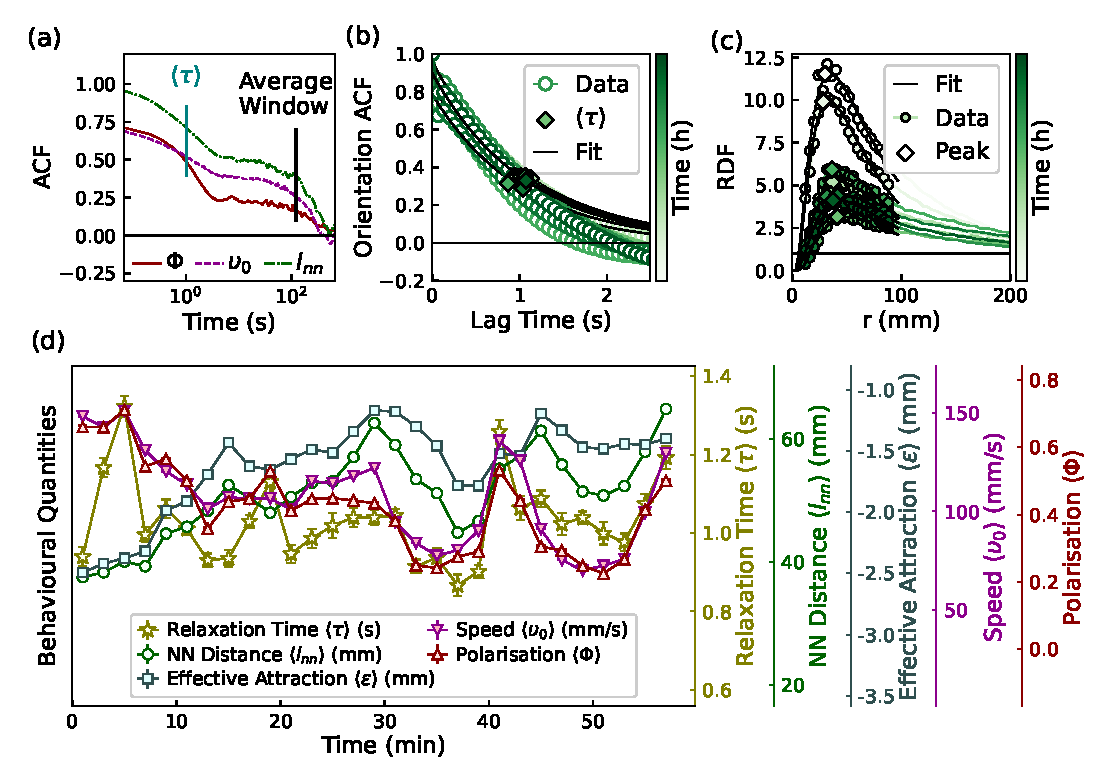
\includegraphics[width=\linewidth,outer]{descriptor-many-fish}
  \caption[The behavioural descriptors of 50 zebrafish]{
  	(a): The auto--correlation function of the polarisation and average speed of the fish group.
	(b): The auto--correlation function of the orientations of fish.
	(c): Sequence of radial distribution functions with increasing time: at early times (top curves) the fish are clustered together so that the peak is large; at later times (bottom curves) the local density decreases and so does the peak height.
	(d): The time evolution of the averaged {\descriptors} for 50 {\smallfish} fish. Each point corresponds to the average value in 2 minutes.
	The error bars illustrate the standard error values.
  }
  \label{fig:descriptor-many-fish}
\end{SCfigure}

\section{Conclusion}

\end{document}

\documentclass[11pt,twoside]{report}
\usepackage{preamble}
\graphicspath{{../img/ch5/}}
\setcounter{chapter}{5}


\begin{document}

\chapter{Analysing The Zebrafish Behaviour}
\label{chapter:fish_analysis}


\section{Introduction}


Some descriptive quantities such as density distribution, average speed, and degree of polarisation would also be presented. Inspired by the soft--matter community, I also calculated the temporal and spatial correlation functions to characterise the system. These quantities and correlation functions will serve as the final target for modelling the zebrafish in the next chapter.


\section{From Locations to Trajectories}


\subsection{Removing Overlapped Particles}
\label{section:overlap}

I used linear programming method to remove overlapped coordinates. The overlap happened if different parts of the fish matched different kernels.

Supposing there are $N$ particles in total, and we wish to find $K$ non--overlapping particles, where each particle has an uncertainty value of $e_i$. The task can be written as a linear programming problem with quadratic constrains as follows:

\begin{equation}
\begin{aligned}
	\textrm{Minimize} && \sum_i{e_i x_i} \\
	\textrm{Subject to} && d_{12} x_1 x_2 \le \sigma \\
	&& d_{13} x_1 x_3 \le \sigma \\
	&& \vdots  \\
	&& d_{ij} x_i x_j \le \sigma \\
	&& \sum_i{x_i} = K
\end{aligned}
\end{equation}

\noindent where $d_{ij}$ is the distance between particle $i$ and $j$, $\sigma$ is the diameter of the non--overlapping hard core of each particle, and $K$ is the total number of particles. The solution to above cost function and constrains can be effectively solved by the CPLEX optimisation package. (SITE IBM).\marginfootnote{As a recent development, IBM announced a faster version of CPLEX using the deep neural network to perform the same optimisation task.}

An alternative choice is to apply a greedy algorithm, to always remove the worst match until there is no overlap. The greedy algorithm is much easier to implement, and can sometimes find good solutions. However, the linear programming method will find the global minimum of the cost, therefore being selected in my study.

The overlapping resolve method introduced in this subsection can be extended beyond tracking animals. In fact, it can be very helpful to refine the particle tracking result for colloidal experiments, where the traditional algorithm might give overlapping coordinates because of intensity noises. In the colloidal experiment, the error term can be the inverse of the fluorescent intensity (to favour brighter centres) or the response to a kernel function (to favour a particular shape).

\subsection{Linking Positions to Trajectories}
\label{section:link}

With the positions of all the fish, one can study the \emph{structure} of the fish group. However, extra work needed to be carried out in order to obtain the \emph{dynamic} of the system. Because the velocities of each fish is needed to calculate the dynamical quantities like the spatial/temporal velocity correlation function, which is used to extract the correlation length and the leadership relationship. To get the velocities, it is necessary to link the positions, at different time points, into trajectories. The concept is illustrated in.

% words and figure to illustrate a linking procedure.

The linking procedure requires a prior knowledge of the dynamic of the system under study. For example, the dynamic of colloidal particles is known to be Brownian, whose.

% introduce the CG linking procedure.

However, the situation for the fish is a bit different: we don't really know the dynamic of the fish, hence the cost function to minimise in the linking procedure is a bit unclear.

To tackle the situation, to my best knowledge, one can start with very simple assumptions. One possible choice is the constant speed.

% introduce Ouellette's paper.

Implementing the algorithm, I obtained some very short trajectory segments. These segments can be extended further following

% introduce Xu's idea and the global optimisation procedure.

Practically, enumerating all the possible linking choices can take a very long time. So

% talk about the heuristic to restrain dt dx.

Pass



\subsection{Analysing the Trajectories}

Several quantities were calculated to analyse the trajectories of the fish, and the calculations are generic for both 2D and 3D trajectories. Therefore these quantities will also be used in Chapter~\ref{chapter:fish_3d}.

\begin{SCtable}
	\begin{minipage}[b]{\linewidth}
	\centering
		\begin{tabular}{c l c r}
			\toprule
		    Symbol & Name & Unit & Comment \\
		    \midrule
		    $v_0$ & Speed & mm/s & Average over different fish\\
		    {\dnn} & Nearest Neighbour Distance & mm & Average over different fish\\
		    $\Phi$ & Polarisation &  1 & Larger = ordered movement\\
		    $\left\langle \cdot \right\rangle$ & Average operator  & &  Time average\\
		    {\mtau} & Relaxation time & s & The relax of fish orientation \\
		    {\meps} & Effective Attraction & 1 & Smaller = more cohesive\\
		    {\mlp} & Persistence Length & mm & Defined as {\mspd}{\mtau} \\
		    $\kappa$ & Reduced Persistence Length & 1 & Defined as {\mlp} / {\mdnn} \\
		    \bottomrule
		\end{tabular}
	\end{minipage}
	\label{tab:behaviour-quantities}
	\caption{A summary of the variables used to describe the fish behaviour.}
  \label{table:geometry}
\end{SCtable}


\subsection{Refine the Trajectories}

The 3D positions obtained from the tracking system can be linked into trajectories described in section \ref{section:link}. The linked trajectories are good, thanks to the predictive linking method and the subsequent relinking, but it is still possible to further optimise the trajectories. The idea is to re--incorporate the information of the 2D features and cameras into the trajectories.

\subsection{Accuracy Evaluation}

I evaluated the accuracy of the tracking method with the simulated data. Typically, I generated the trajectories of 50 simulated fish inside a container. Then I use the software \emph{Blender} (version 2.91.0 on Ubuntu 20.04) to render the movement of the fish as animations, with multiple cameras. The result movies looks very similar to my experimental videos, in terms of the local fish density and the speed. This similarity ensured the accuracy that I assessed from the simulation movie is valid for my experimental data.


\section{From Trajectories to Behaviour}

\subsection{The Static Features}

\subsection{The Dynamical Features}


\section{The Behaviour of Zebrafish in 2D}


\section{The Behaviour of Zebrafish in 3D}

The 3D tracking yields the positions of the fish, whose discrete time derivative gives the velocities. From these two quantities, we calculate three global descriptors to characterise the behaviour of the fish: the average speed, the polarisation, and the nearest neighbour distance. The average speed is defined as $v_0 = 1/N \sum{|\vi|}$ where $i$ runs over all the tracked individuals. 

For experiments with more than one fish, the polarisation $\Phi$ was commonly used to characterises the alignment of the velocities. It is defined as the modulus of the average orientation, written as \cite{attanasi2014pcb},
$\Phi = 1/N \left| \sum{({\vi}/{| \vi |}}) \right|$ where $i$ runs over all the individuals. Large polarisation ($\Phi \sim 1$) signifies synchronised and ordered movement, while low polarisation indicates decorrelated, random movement. The polarisation is sometimes referred to as the ``order parameter'' by physicists, since it is a measure of the order of the fish dynamic. We say a group of fish have \emph{ordered} movement if they are swimming towards the same direction.\marginfootnote{If we think of the moving direction of the fish as little spins of a magnetic system, then the polarisation is mathematically equivalent to the average magnetization per spin.}

The local density of the group also plays important roles in the collective behaviour. The local density can be probed by the nearest neighbour distance, which is noted as {\dnn} in this thesis. For a fixed number ($N$) of fish in a fixed sized environment (with volume $V$), their overall number density is constant (being $N/V$). However, the groups with smaller {\dnn} is more cohesive.


\subsection{A Single Fish}
\label{section:fish_1_3d}


Figure~\ref{fig:density_3d_fish_1} shows the spatial distribution of one fish in the observation tank. It is obvious that the fish tend to stay in the bottom of the tank. It is a typical fish behaviour when they were subjected to a new environment, and it is known as the ``depth preference''.
Nevertheless, the distribution of the $X$ components of the coordinates is symmetric, which suggests the fish do not have a preferred location to stay in the tank.


\begin{SCfigure}
  \includegraphics[width=\linewidth,outer]{density-one-fish}
  \caption[The 3D spatial distribution of one fish]{The spatial distribution of one adult zebrafish. The top panel shows the joint distribution of the $Y$ coordinates and $Z$ coordinates of the fish positions. The bottom panel shows the distributions of the $X$ coordinates, the planar radius ($R$) and the $Z$ coordinates. The distribution of the ideal gas in the tank was given as a reference.}
  \label{fig:density_3d_fish_1}
\end{SCfigure}

From the fish trajectories, we can also calculate their speed and orientations in each from. These time series also offer the typical time scale of speed changing and orientation relaxing.


\subsection{A Pair of Fish}
\label{section:fish_2_3d}

The spatial distribution of 2 zebrafish were presented in Fig~\ref{fig:density_3d_fish_2}. The behaviour of 2 fish is similar to that of one fish. Namely, the fish tend to be around the bottom of the tank.

\begin{SCfigure}
  \includegraphics[width=\linewidth,outer]{density-two-fish}
  \caption[The 3D spatial distribution of two fish]{The spatial distribution of two adult zebrafish. The top panel shows the joint distribution of the $Y$ coordinates and $Z$ coordinates of the fish positions. The bottom panel shows the distributions of the $X$ coordinates, the planar radius ($R$) and the $Z$ coordinates. The distribution of the ideal gas in the tank was given as a reference.}
  \label{fig:density_3d_fish_2}
\end{SCfigure}

The fish interaction can be probed by the relative distribution of the neighbours of the fish. 


\subsection{Three Fish}
\label{section:fish_3_3d}

The spatial distribution of 2 zebrafish were presented in Fig~\ref{fig:density_3d_fish_3}. Being similar to the one fish and two-fish case, a group of three fish presents the depth preference.

\begin{SCfigure}
  \includegraphics[width=\linewidth,outer]{density-three-fish}
  \caption[The 3D spatial distribution of three fish]{The spatial distribution of three adult zebrafish. The top panel shows the joint distribution of the $Y$ coordinates and $Z$ coordinates of the fish positions. The bottom panel shows the distributions of the $X$ coordinates, the planar radius ($R$) and the $Z$ coordinates. The distribution of the ideal gas in the tank was given as a reference.}
  \label{fig:density_3d_fish_3}
\end{SCfigure}

\subsection{Many Fish}
\label{section:fish_many_3d}

We studied the behaviour of 50 fish with two different age groups, the {\smallfish} whose age is between 6 months old to 1 year, and the {\bigfish} whose age is beyond 1 year.

The behavioural quantities, as I summarised in Table~1, is shown in Fig~\ref{fig:descriptor-many-fish}.

\begin{SCfigure}
  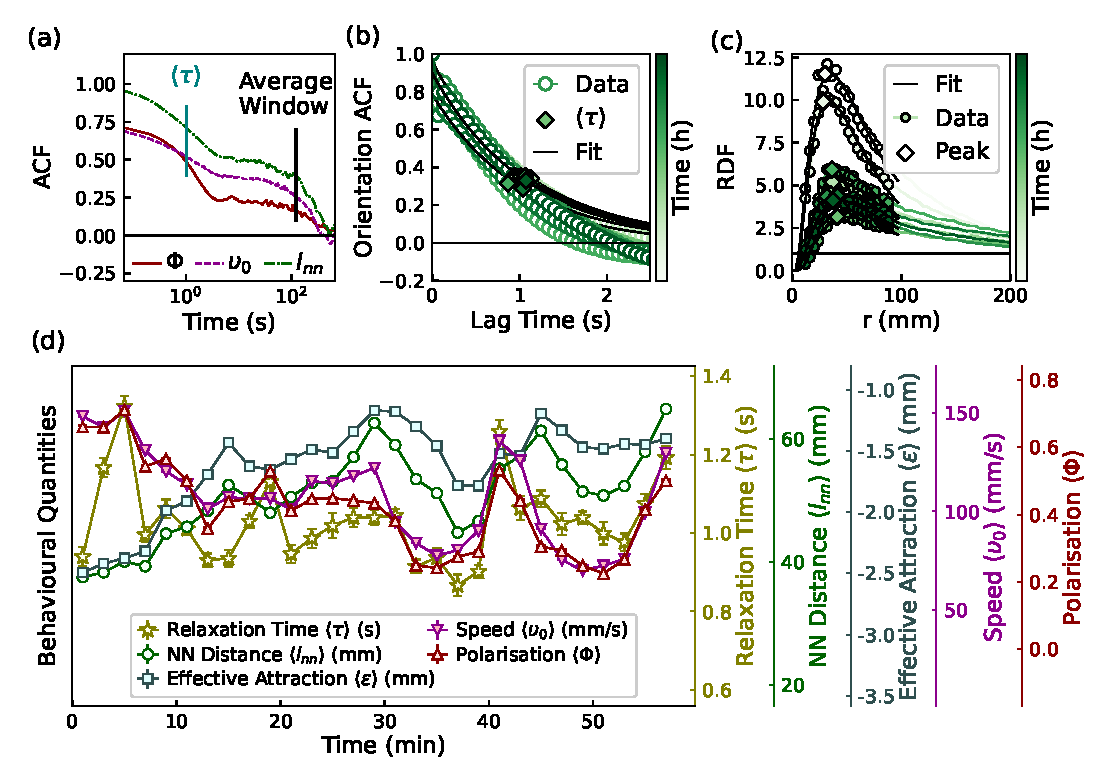
\includegraphics[width=\linewidth,outer]{descriptor-many-fish}
  \caption[The behavioural descriptors of 50 zebrafish]{
  	(a): The auto--correlation function of the polarisation and average speed of the fish group.
	(b): The auto--correlation function of the orientations of fish.
	(c): Sequence of radial distribution functions with increasing time: at early times (top curves) the fish are clustered together so that the peak is large; at later times (bottom curves) the local density decreases and so does the peak height.
	(d): The time evolution of the averaged {\descriptors} for 50 {\smallfish} fish. Each point corresponds to the average value in 2 minutes.
	The error bars illustrate the standard error values.
  }
  \label{fig:descriptor-many-fish}
\end{SCfigure}

\section{Conclusion}

\end{document}

\documentclass[11pt,twoside]{report}
\usepackage{preamble}
\graphicspath{{../img/ch6/}}
\setcounter{chapter}{5}

\begin{document}

\chapter{Modelling Zebrafish}
\label{chapter:fish_model}


\epigraph{人相忘乎道术}{庄子}


\section{Introduction}

In this chapter we will study the behaviour of the zebrafish with the help of computer simulation. The goal of the simulation is to reproduce the experimental results from chapter~\ref{chapter:fish_2d} to chapter~\ref{chapter:fish_analysis}.
We will use the Monte-Carlo simulation to study a system in equilibrium, in order to reproduce the spatial distribution of the fish under the influence of the boundary, the gravity, as well as the pairwise interaction.
In addition, we will use a dynamical simulation to study an agent-based\marginfootnote{
The dynamical simulation is similar to the Brownian dynamics simulation for the liquid, where all the particles were updated according the force exerted on them. It's different from the Monte-Carlo simulation where the particles are moved randomly.
The moving individuals in the model can take different names, like the ``particles'', ``animals'', and ``agents''. The term ``agents'' will be used in this chapter for consistency.
} active matter model, in order to recreate the dynamical feature of the fish group in the experiments.
%The purpose of these simulations is to understand and explain the observed zebrafish behaviour, so that we could get more insights into its nature. 
%In particular we focus on the distribution of the density, as well as the order of the dynamics.

The density distribution of the fish was strongly affected by the presence of the boundary, as the fish were physically constrained in the tank.
For the 3D experiment, the distribution of the fish was also affected by an ``effective gravity'', as well as the holes drilled on the tank. These environmental factors can be treated as external fields affecting the fish. In addition to these external factors, the fish-fish interaction will also change their distribution.
With the Monte-Carlo (\gls{MC}) simulation techniques, we can study these effects individually. By doing so, we implicitly tested the idea of mapping active matter system to an equilibrium counterpart, where the non-equilibrium feature of the system, the activity, was summarised by an effective temperature\marginfootnote{
This ``effective equilibrium'' picture is supported by the exponential decay of the excess distribution function shown in section~\ref{section:fish_1_3d}, as the decay suggests the Boltzmann-like distribution commonly seen in equilibrated systems.
} \cite{palacci2010, klongvessa2019}.

For a group of fish, the order of their dynamics, captured by the polarisation value (Eq.~\ref{eq:polarisation}), correlates robustly with a non-dimensional value \gls{kappa}, the ratio between the persistence length (\gls{lp}) and the nearest neighbour distance (\gls{lnn}).
Such a correlation suggests the local density and the persistence motion of the fish dominated the polarisation of the system.
Since the persistence motion is a proxy to the \emph{activity} of the fish, the entire group of 50 zebrafish is behaving like an alignment dominated active matter system (section~\ref{section:active-phase}).
To confirm the similarity of a group of zebrafish, and a model active matter system, we will use the dynamical simulation method to simulate the famous active matter model, the Vicsek model.
To get a good fit between the model and the experiments, we will have to modify the Vicsek mode and consider the orientational inertia of the fish.
The fitting of the model and the experimental result suggests the existence of the effective alignment interaction among the fish. And the changing states of the fish could be understood as a change of the noise level for the model.


\section{Simulation Methods}


\subsection{General Idea}

If we think of fish as a collection of agents following pre-defined movement rules, we could reproduce the movement of the fish with the computer simulation. Formally, we call a collection of agents a \emph{system}. And the system can change its (microscopic) states over time.
By observing the system for a long time, we could obtain the trajectory of the system, and then calculate the quantities that we are interested in (see chapter~\ref{chapter:fish_analysis} for examples). Such process is summarised in the following algorithm (Algorithm~\ref{alg:simulation}).
During the simulation, the system change its states under some constraints. For example, the constraints could be a controlled noise level (\gls{beta}), a constant number density (\gls{rho}), and a fixed total number (\gls{N}) of agents.


\begin{algorithm}
	\KwData{Constraints $\{ \beta, \rho, N, \dots \}$}
	\KwResult{Trajectory}
	System $\gets$ initial microscopic state with $\{ \beta, \rho, N, \dots \}$\;
	\Repeat{System is stable, and forgets the initial microscopic state}{
		change the microscopic state of the system with $\{ \beta, \rho, N, \dots \}$
	}
	Trajectory $\gets \emptyset$\;
	\Repeat{
		The statistics are good enough
	} {
		change the microscopic state of the system with $\{ \beta, \rho, N, \dots \}$\;
		Put current state in Trajectory\;
	}
\caption{The Simulation Procedure}
\label{alg:simulation}
\end{algorithm}

\subsection{Monte-Carlo Simulation}

There are multiple ways to change the state of the system in algorithm~\ref{alg:simulation}. In a seemly arbitrary fashion, we could change the state of the system randomly, and reject some states that is unlikely to happen. This method is termed ``Monte-Carlo'' (MC) simulation, and the acceptance ratio were often determined by the Metropolis algorithm. Typically, the acceptance ratio from state $\zeta$ to $\nu$, \gls{acc}, is written as

\[
	A(\zeta \rightarrow \nu) = \left\{
		\begin{array}{ll}
			\exp\left(-\beta(E_\nu - E_\zeta)\right)
			& \mbox{if $E_\nu - E_\zeta > 0$}\\
			1 & \mbox{otherwise.}
		\end{array}
	\right.
\]

\noindent And the values of $E_\nu$ and $E_\zeta$ represent the energy values of state $\nu$ and $\zeta$, respectively. The value $\beta$ is the inverse temperature. The smaller $\beta$ value is, the higher the temperature, and the larger randomness the system exhibits.

With MC simulation, it is easy to constrain the agents in the fish tank, by setting $E = \infty$ once an agent is outside the tank.\marginfootnote{
Operationally, we reject the states if any agent is outside the fish tank.
} In addition, the effect of external fields, like gravity, can be added easily to the simulation. However, due to the lack of ``true'' dynamics in the MC simulation, we will not have access to the velocities of the system. Hence, this simulation method is only used to model the spatial distribution of the zebrafish.


\subsection{Dynamical Simulation}


Another way to change the state of the system is to integrate the \emph{equation of motion} of all the agents. For animals, the equations to be integrated represent the behavioural rules of the agents.
Being different from the conventional molecular dynamics simulation or mesoscale simulations \cite{allen2017}, the simulation of animal behaviour often incorporates more eccentric rules, such as a fixed vision zone\cite{couzin2002, yigit2020}, and an attraction to the group centre \cite{reynolds1987}. Generally, the updating rules for the agents could be described by the following equation,

\begin{equation*}
\begin{split}
	\mathbf{v}_{i}^{t+1}
	&= \mathcal{B} [\mathbf{v}_{i}^t] \\
	\mathbf{x}_i^{t+1}
	&= \mathbf{x}_i^{t} + \mathbf{v}_i^{t+1},
\end{split}
\end{equation*}

\noindent where the operator $\mathcal{B}$ encodes all the behavioural rules of the animals. By changing the coordinates and velocities of all the agents simultaneously, we change the state of the system (Algorithm~\ref{alg:simulation}).


\section{The Distribution of the Density}
\label{section:simulate-density}

In this section we will model the spatial distribution of the fish in the 3D experiment. The simulation will illuminate the effects of the environmental factors, such as the fish tank and the gravity. By comparing with the experimental density distribution, we can get phenomenological parameters such as the effective temperature, to describe the behaviour of the fish.



\subsection{The Effect of the Tank}
\label{section:sim-mc-tank}

The 3D geometry of the tank confining the zebrafish was determined in section \ref{section:system_3d}, and the shape of the tank can be expressed as,

\begin{equation*}
	z = c r^2,	
\end{equation*}


\noindent where $c=0.74 m^{-1}$ when both $r$ and $z$ were expressed in the unit of meters. The volume (\gls{vol}) of the tank can be calculated as

\begin{equation*}
	V = \int_{0}^{h}{\pi \frac{z}{c}} dz
	  = \frac{\pi h^2}{2 c},	
\end{equation*}


\noindent where $h$ is the height of the tank, the vertical distance between the water surface and the base of the tank. The joint probability density function (PDF) of random points, being uniformly distributed inside the tank, is written as,

\begin{equation*}
	f(x, y, z) = V^{-1} = \frac{2c}{\pi h^2}.		
\end{equation*}

\noindent The joint PDF of the uniform distribution can be expressed in the spherical coordinates as,

\begin{equation}
	f(\theta, r, z) = \frac{2c}{\pi h^2} r,
\label{eq:density-pdf-tank}
\end{equation}

\noindent where $\theta$ is the azimuthal angle, $r = \sqrt{x^2 + y^2}$ is the radius in $XY$ plane.  From the expressions above, we can calculate the marginal distribution of $r$ and $z$ coordinates:

\begin{equation}
\begin{split}
	f_R(r) &= \int_0^{2\pi}{d \theta} \int_{cr^2}^{h}{dz} \; f(\theta, r, z)
		= \frac{4c}{h} r - \frac{4 c^2}{h^2} r^3, \\[2em]
	f_Z(z) &= \int_0^{2\pi}{d \theta} \int_0^{\sqrt{z/c}}{dr} \; f(\theta, r, z) 
	= \frac{2}{h^2} z.
\end{split}
\label{eq:dist-tank}
\end{equation}

\noindent The analytical result (Eq.~\ref{eq:dist-tank}) is checked against the numerical sampling of random points inside the tank, as shown in Fig.~\ref{fig:dist-tank}. These PDFs can be used as comparison for the distribution of real fish data, as presented in section~\ref{section:observe-3d-result}. The experimental distribution of the fish is very different from the ideal gas distribution.

\begin{SCfigure}
  \includegraphics[width=\linewidth]{density-tank}
  \caption[The 3D geometry of the experimental fish tank]{
  The marginal probability density distribution of points sampled uniformly inside the experimental fish tank.
  Left: the distribution the planar radius $r$.
  Right: the distribution of the $z$ component of the points.
  }
  \label{fig:dist-tank}
\end{SCfigure}


\subsection{The Effect of the ``Gravity''}
\label{section:sim-mc-gravity}

From the results presented in section~\ref{section:observe-3d-result}, it is evident that the zebrafish will be affected by an ``effective gravity'', because of their depth preference behaviour.
This effective gravity is similar to 
As a first attempt, we could calculate the density distribution of ideal gas particles in equilibrium, with an Boltzmann weight $\exp(-\beta z)$ to capture the effect of the gravity.
The \emph{partition function} (\gls{Z}) of the system is written as,

\begin{equation*}
	Z = \int_0^h \pi \frac{z}{c} \exp(-\beta z) dz
      = \frac{\pi (1 - \exp(-\beta h) (1 + \beta h))}{c \beta^2}.
\end{equation*}

\noindent With the partition function, we could then calculate the joint probability density function of the ideal gas, in the spherical coordinate system (similar to Eq.~\ref{eq:density-pdf-tank}).

\begin{equation}
	f(\theta, r, z)
	= \frac{r \exp(-\beta z)}{Z}
	= \frac{c \exp(-\beta z) r \beta^2}
	{\pi(1 - \exp(-\beta h)(1 + \beta h))}
\label{eq:density-pdf-gravity}
\end{equation}

\noindent where $\beta = 1 / (k_B T)$ is the inverse temperature. For a physical systems in equilibrium, the vale of \gls{beta} relates to the real temperature measured by a thermometer. However, the value of $\beta$ for the fish only controls the level of randomness of the system, without a concrete physical meaning. From the function $f(\theta, r, z)$, we can calculate the distribution functions $f_R(r)$ and $f_Z(z)$:

\begin{equation}
\begin{split}
	f_R(r) &= \int_0^{2\pi}{d \theta} \int_{cr^2}^{h}{dz} \; f(\theta, r, z)
		= \frac{
			2 c \left(
					\exp \left( \beta (h - c r^2) \right) - 1
				\right) r \beta
		}{
			\exp(\beta h) - \beta h - 1
		}, \\[2em]
	f_Z(z) &= \int_0^{2\pi}{d \theta} \int_0^{\sqrt{z/c}}{dr} \; f(\theta, r, z) 
	= \frac{\exp(-z \beta) z \beta^2}{
		1 - \exp(-\beta h) (1 + \beta h)
	}.
\end{split}
\label{eq:dist-gravity}
\end{equation}

\noindent The results from Eq.~\ref{eq:dist-gravity} were checked against the Monte-Carlo simulation results, as shown in Fig.~\ref{fig:dist-gravity}. With the increase of $\beta$, hence the decrease of temperature, the agents were pushed towards smaller $z$ values and $r$ values. By ``fitting'' the experimental results with the analytical results from Eq.~\ref{eq:dist-gravity}, and setting $\beta$ as a free parameter, we could obtain the effective temperature for the fish.
%A systematic study of the change of the effective temperature could give us a more systematic understanding of the depth preference of the zebrafish. For instance, the fitting parameter $\beta$ could be interpreted as the ``fear'' perceived by the fish.

\begin{SCfigure}
  \includegraphics[width=\linewidth]{density-gravity}
  \caption[The distribution of ideal gas in the tank subjected to gravity]{The marginal probability density distribution of ideal gas particles sampled uniformly inside the experimental fish tank, where the particles were subjected to the gravity field. Left: the distribution the $z$ component. Right: the distribution of the $r = \sqrt{x^2 + y^2}$. The scatters were result of Monte-Carlo simulations, and the solid lines were from Eq.~\ref{eq:dist-gravity}.}
  \label{fig:dist-gravity}
\end{SCfigure}


\subsection{The Effect of the Holes}
\label{section:sim-mc-holes}

In our 3D fish observation experiments, the holes on the tank disrupted the density distribution of the fish. This disruption makes the result in Eq.~\ref{eq:dist-gravity} very different from the distribution of the fish, as shown in section~\ref{section:holes}. To mimic such effect, we could model holes as an extra field, with the following form,

\begin{equation}
	H(r, z) = q
		\sum_i{\frac{
		\left[
			(r - r_i)^2 + (z - c r_i^2)^2
		\right]^{-2}
		}{r_i}},
\label{eq:energy-holes}
\end{equation}

\noindent where $r_i$ represents the location of the holes on the tank. Specifically, there are three sets of holes (Fig.~\ref{fig:density-holes}), located at $r_1=96$ mm, $r_2=213$, and $r_3=327$ mm. The denominator ($r_i$) in Eq.~\ref{eq:energy-holes} represents the fact that equal amount of holes were drilled on the circles. So that the larger circles will have less holes per unit length. The factor \gls{q} controls the strength of the repelling interaction between the fish and the holes.

Calculating the corresponding density distributions, \gls{pdfr} and \gls{pdfz}, analytically is difficult, but we can estimate the density distribution with the Monte-Carlo simulation. Figure~\ref{fig:dist-holes} shows the result of the simulation. As expected, the distribution $f_R(r)$ appears bimodal with a locally minimum $q$ value at the location $r = r_1$.

\begin{SCfigure}
  \includegraphics[width=\linewidth]{density-holes}
  \caption[The effect of the holes on the density distribution]{
  The effect of the holes on the density distribution of ideal gas in the fish tank subjected to gravity field.
  (a): the distribution the $z$.
  (b): the distribution of the $r$.
  The colour of the lines indicates the strength of the repulsive interaction of the holes on the tank. The simulation was carried out with parameter $\beta=50$, where $7.5 \times 10^{6}$ coordinates were sampled.
  }
  \label{fig:dist-holes}
\end{SCfigure}


\subsection{The Effect of Pairwise Interaction}
\label{section:sim-mc-interaction}


\marginpar{
\centering
\includegraphics[width=\marginparwidth]{fit-gr}
\captionof{figure}{Fitting the $u(r)$ of fish with Eq.~\ref{eq:fit-ur}.}
\label{fig:fit-ur}
}

The simulations in section~\ref{section:sim-mc-tank} to \ref{section:sim-mc-holes} treat the agents as ideal gas particles, without any interaction between the agents. This is not realistic, since the $g(r)$ of the zebrafish exhibits characteristic features (Fig.~\ref{fig:structure-3d} (c) in section~\ref{section:analysis-structure-3d}).
In order to enable the agents to behave more like the zebrafish during the Monte-Carlo simulation, we added an effective agent-agent interaction energy term based on the pairwise distances of the agents. The effective potential energy\marginfootnote{
Notice the logarithm of $g(r)$ is $-\beta u(r)$ for equilibrium systems. Here we ignored the $\beta$, and we controlled the strength of the pairwise interaction with parameter $q$.
The reason for our choice is that we are only interested in the approximated shape of $u(r)$, which makes the fish forming a coherent group, rather than the exact analytical form of $u(r)$.
}
, \gls{ur}, is written as,

\begin{equation*}
	u(r) = -p \log\left[ g(r) \right]
\end{equation*}

\noindent where \gls{p} is a free parameter that determines the contribution of the interaction between the agents. To parameterise the experimental $u(r)$, we fitted it with function

\begin{equation}
	u(r) = \log(a_1) - \log(2)\left[
		\frac{
			\log(1 + 2a_2(r-a_3)/a_4)
		}{a_2}
	\right]^2,
\label{eq:fit-ur}
\end{equation}


\noindent where $a_1$ - $a_4$ are fitting parameters. Figure~\ref{fig:fit-ur} shows the fitting result, where the potential energy took a minimum at the location of nearest neighbour distance.
We can incorporate this pairwise interaction into the energy form during the Monte-Carlo simulation, to study its effects. Formally, the energy of the system could be written as,


\begin{equation}
	E = \left\{ \begin{array}{ll}
		\sum_i\left[
			z_i + H(r_i, z_i) + 
			\sum_{j \neq i}{u(d_{ij})} 
			\right]
			&  \mbox{if $c r_i \le z_i < h$}\\
		\infty & \mbox{otherwise}
	\end{array}\right.
\label{eq:model-density}
\end{equation}



\noindent where the coordinate of agent $i$ is $(x_i, y_i, z_i)^\top$, with $r_i = \sqrt{x_i^2 + y_i^2}$. The condition ($c r_i \le z_i < h$) ensures the agents staying in the boundary. This ``energy'' is a mixture of the effective gravity\marginfootnote{
Notice we implicitly transformed the height of the fish ($z_i$) to the potential energy in an effective gravitational field in Eq.~\ref{eq:model-density}.
}, the repulsive holes, and the pairwise interaction, and it is controlled by parameter $p$ and $q$.
When both $p$ and $q$ are equal to zero, the agents behave like ideal gas in the tank subjected to the effective gravity. But tuning the value of $p$ and $q$, we increase the effect of the pairwise interaction and the holes.


The effect of the pairwise interaction of the fish on the density distribution is shown in Fig.~\ref{fig:dist-interaction}, where we fixed the value of $q$ (which controls the strength of the fish-hole interaction) to be $0$, and set $\beta=0.1$. These parameters correspond to the condition where the effects of both the gravity and the holes could be ignored.
When the value of $p$ is small, so that the interaction among the agents are weak, the system behaves like ideal gas particles under gravity, described by Eq.~\ref{fig:dist-interaction}. When the value of $p$ was gradually increased from $10^{-2}$ to 1, the fish tend to aggregate near the bottom of the tank in the centre.


Notably, the further increase of $p$ would change the density distribution of the fish in a different fashion. As the value of $p$ increased from 1 to 10, the fish are more frequently appear at higher $r$ and $z$ values. Such non-monotonic behaviour could be understood by carefully examining the effective interaction potential $u(r)$ of the agents.
Typically, the interaction potential would constrain the agents to form a coherent cluster, to mimic the observed structure of the fish group (section~\ref{section:analysis-structure-3d}). And the size of the cluster would decrease, with the increase of $p$, as shown in Fig.~\ref{fig:fish-cluster}.
For smaller clusters, they would be able to explore the ``corner'' of the fish tank, where both $r$ value and $z$ value are high.
On the other hand, the large clusters would have to deform its shape, paying extra energy cost, so that they could enter the corner region.
Therefore, the agents with stronger pairwise interaction would explore more space in the tank, presenting higher chance to appear in regions where $r$ and $z$ values are high.


\marginpar{
\centering
\includegraphics[width=\marginparwidth]{fish-cluster}
\captionof{figure}{The parameter $p$ controls the size of the group.}
\label{fig:fish-cluster}
}


\begin{SCfigure}
  \includegraphics[width=\linewidth]{density-interaction}
  \caption[The effect of the pairwise interaction on the density distribution]{
  The effect of the pairwise interaction among the agents, on their density distribution.
  (a): the distribution the planner radius $r=\sqrt{x^2 + y^2}$ of the agents' coordinates.
  (b): the distribution of the $z$ component of the agents' coordinates.
  The colour of the solid lines indicates the strength of the pairwise interaction of the fish. The dashed lines corresponds to the result where $p=0$. The simulation was carried out with parameter $\beta=0.1$, where $5 \times 10^{5}$ coordinates were sampled.
  }
  \label{fig:dist-interaction}
\end{SCfigure}



\subsection{Comparison to Experimental Data}


We used the energy term in Eq.~\ref{eq:model-density} to simulate the equilibrium density profile of the agents, and compare the results with our experimental data obtained in chapter~\ref{chapter:fish_3d}. By tuning the parameters, typically the values of $\beta$, $q$, and $p$ manually, we can generated simulation result that is similar to the experimental results. The fitting result is shown in Fig.~\ref{fig:model-density}.

For the distribution of one fish in the tank, the fitting results suggests an effective inverse temperature of $\beta = 200$, and the strength of the fish-hole interaction of $a = 2\times 10^{-10}$, as presented in Fig.~\ref{fig:model-density} (a) and (b). By decreasing the value of $\beta$ to 45, and incorporating the fish-fish interaction with $p = 10$, we could model the density profile of 2 fish, as shown in Fig.~\ref{fig:model-density} (c) and (d). There is a slight mismatch between the experiment and the model, which might related to the non-equilibrium nature of the fish, which is absent in our Monte-Carlo simulation.
 
 To match the density profile of 50 fish, the value of $\beta$ needs to be further decreased to 0.1, while keeping the $q$ and $p$ values unchanged. However, the match between the experimental data and the model is poor. In fact, the bimodal distribution of $f_Z(z)$ of 50 fish, shown in Fig.~\ref{fig:model-density} (f), indicates the presence of multiple states, as reported in section~\ref{section:change-states-3d}. To take multiple states into consideration, we will need to overlay simulation results from multiple systems with different parameters. Such a complex simulation is beyond the scope of this chapter.
  
Even though the fitting between the experimental density distribution and that from the Monte-Carlo simulation is not very good, the result is in accordance with our previous discussion in chapter~\ref{chapter:fish_2d} and \ref{chapter:fish_3d}. Namely, when the number of fish is small, the interaction between the fish and the environment (gravity and holes) is significant. Such importance could be translated to a high $\beta$ value in our model. For a group of 50 fish, the fish-fish interaction dominates their behaviour, corresponding to a low $\beta$ value.


\begin{SCfigure}
  \includegraphics[width=\linewidth]{model-density}
  \caption[Comparing the density distribution of the fish and the model]{
  The comparison of the density distribution of fish with the model described by Eq.~\ref{eq:model-density}. The data points represent the experiment measurements, and the solid lines were calculated from the Monte-Carlo simulation.
  (a): the distribution the $z$ from 1 fish.
  (b): the distribution of the $r$ from 1 fish.
  (c): the distribution the $z$ from 2 fish.
  (d): the distribution of the $r$ from 2 fish.
  (e): the distribution the $z$ from 50 fish.
  (f): the distribution of the $r$ from 50 fish.
  }
  \label{fig:model-density}
\end{SCfigure}

\subsection{Limitation of the Model}

It is important to stress the limitation of our model to describe the behaviour of the fish. Importantly, our Monte-Carlo simulation essentially assumed the fish were in equilibrium states, in which detailed balance is satisfied \cite{newman1999}. This is not true for the zebrafish, as a group of fish constantly dissipate their biological energy to swim. Visually, the movement of fish is very different from the movement of atoms in the gaseous or fluidic phases. For example, if we play the movie of swimming fish backwards, it looks very unnatural. In addition, the interaction between the fish and the environment is speculative. Here we assumed the tank is a hard boundary, and the depth preference of the fish were described by an effective gravity, and the holes have an effective parabolic repelling interaction. And these assumptions may not be accurate, which requires scrutiny.


\section{The Order of the Dynamic}
\label{section:simulate-dynamics}

The movement of a group of fish can exhibit two visually different states. The fish may exhibit \emph{ordered} movement, swimming in the same moving direction, with a high polarisation ($\Phi$) value. Alternatively, the fish may exhibit random movement, where they swim in different directions. The switch between random movement and ordered movement is observed for a group of fish in Chapter~\ref{chapter:fish_analysis}.

Intuitively, the ordered movement is a special state comparing with its random counterpart. And animals have to somehow make something happen, to effectively align with each other and share the same moving direction. In this section, we will try to model this process.


\subsection{The Vicsek Model}
\label{section:vicsek-model}


The Vicsek model is a very simple active matter model for the dynamics of the animals \cite{vicsek1995}. Essentially, the agents align with nearby neighbours in the model, leading to the ordered movement.
The Vicsek model and its derivatives enjoyed considerable success in describing the collective behaviour of animals. Typically, the equation of motion for the Vicsek model is written as \cite{vicsek1995},

\begin{equation}
\begin{split}
	\mathbf{v}_{i}^{t+1}
	&=
    v_{0} \mathcal{R}_{\eta} \left[\Theta\left(
            \sum_{j \in S_{i}} \mathbf{v}_{j}^t
    \right)\right]
    = \mathcal{V} (\mathbf{v}_{i}^t) \\
	\mathbf{x}_i^{t+1}
	&= \mathbf{x}_i^{t} + \mathbf{v}_i^{t+1},
\end{split}
\label{eq:vicsek}
\end{equation}

\marginpar{
\centering
\includegraphics[width=0.7\marginparwidth]{vicsek-noise}
\captionof{figure}{The scalar noise in the Vicsek model.}
}

\noindent where \gls{vit} represents the velocity of the $i$th agent at time point $t$.
The symbol \gls{si} represents the set containing the neighbours of agent $i$ within the unit distance.
The operator \gls{opnorm} is responsible for normalising a vector to unit norm. The operator \gls{oprot} will rotate a vector randomly around its orientation, adding orientational noise into the system. Such random rotation effectively draws a spherical cap around the vector to be rotated, and the value of \gls{eta} determines the area of this spherical cap.
Formally, the noise is referred to as \emph{scalar noise} in the Vicsek model, as opposed to vectorial noise \cite{pimentel2008}.
We use the symbol \gls{opvicsek} to represent the velocity updating rule of the Vicsek model.


The important parameters for the Vicsek model are the noise ($\eta$) and the number density ($\rho$), when we set the interaction range to one. The noise controls the randomness of the system, and the density controls the neighbour set $S_{i}$ for particle $i$. In addition to $\rho$ and $\eta$, another contributing parameter is the speed of the agents ($v_0$ in Eq.~\ref{eq:vicsek}), but its effect is less significant than $\eta$ and $\rho$. Therefore, we will only focus on $\eta$ and $\rho$.


\begin{SCfigure}
  \includegraphics[width=\linewidth]{phase-vicsek}
  \caption[The phase behaviour of the Vicsek model]{
  The phase behaviour of the Vicsek model. The simulation was performed at different state points, with different density and noise values. The total number of states was $50 \times 50 = 2500$. For each state point, 200 agents were simulated, whose speed was fixed at 0.1. The system was updated $2\times10^4$ steps to reach steady state. The polarisation of the system was recorded in the subsequent $2\times10^4$ steps.
  (a) The time-average polarisation at different states.
  (b) The standard deviation of the polarisation at different states. This value represents the susceptibility of the system.
  The dashed line in both subplots indicates a linear relationship between the transitional density and noise. The end of the dashed line \emph{does not} imply the presence of a critical point.
  }
  \label{fig:phase-vicsek}
\end{SCfigure}

The behaviour of the Vicsek model is presented in Fig.~\ref{fig:phase-vicsek} (a), characterised by the polarisation ($\Phi$) as the order parameter. In the low noise and high density region, the system exhibits ordered behaviour. For the low density and high noise simulations, the agents move randomly with a small $\Phi$ value. Figure~\ref{fig:phase-vicsek} (b) shows the standard deviation of the polarisation from the simulation, whose maximum value indicates the transition between the ordered phase and the disordered phase. In the dilute region, where $\rho < 1$, the transitional density \gls{rhoc} and noise \gls{etac} have a linear relationship, as indicated by the dashed line in Fig.~\ref{fig:phase-vicsek}. Such linear relationship is in accordance with previous 3D numerical simulation results \cite{puzzo2019}.

 

If we try to compare the Vicsek model with the experimental result, the model would fail, as shown in Fig.~\ref{fig:model-dynamics} (a). 
This is because the real zebrafish reached the most random state ($\Phi \sim 0.13$), with a minimum $\kappa$ value of 1.5. That is to say, the fish would have some excess persistence length even in their most random states.
The excess persistence length is expected, as the real fish do not change their orientation at arbitrarily high frequencies. However, this ``minimum persistence length'' does not exist in the Vicsek model, as the Vicsek agents do indeed, change their orientation at a frequency $\sim \infty$, in their most random state, where $\eta = 1$, and $\Phi \sim 0.13$.


\subsection{The Effect of Inertia}
\label{section:model-vicsek-inertia}

One heuristic approach to modify the Vicsek model, so that the model could better match the behaviour of the fish, is to remedy the extreme zigzag movement of the agents in the high noise region. To do so, we could simply let the agents to remember their previous orientations, by rewriting the equation of motion as the following,

\begin{equation}
\begin{split}
	\mathbf{v}_{i}^{t+1}
	&= v_0 \Theta \left[
		(1 - \alpha) \mathcal{V}(\mathbf{v}_i^t) +
		\alpha \mathbf{v}_i^t
	\right]
    \\
	\mathbf{x}_i^{t+1}
	&= \mathbf{x}_i^{t} + \mathbf{v}_i^{t+1},
\end{split}
\label{eq:vicsek-inertia}
\end{equation}

\noindent which is effectively a linear mixture of the Vicsek interaction, noted as $\mathcal{V}(\mathbf{v}_i^t)$, and the original velocity ($\mathbf{v}_i^t$).
The parameter \gls{alpha} controls the ratio between the moving direction from Vicsek interaction to the existing moving direction, and we call it the \emph{inertia}.
When $\alpha$ is zero, the model is reduced to the Vicsek model.
When $\alpha$ is one, all the agents will travel ballistically without any interaction. The trajectories of a single agent with different $\alpha$ values are presented in Fig.~\ref{fig:vicsek-inertia}(b). The agent with moderate $\alpha$ value presents a smooth trajectory, as expected.
Figure~\ref{fig:vicsek-inertia} (a) shows the scaling relationship between the orientational relaxation time and the noise, where $\tau_\mathbf{o} \sim \eta^{-2}$. Such relationship is in accordance with previous proposals \cite{ginelli2016, puzzo2019}. The incorporation of the ``inertia'' ($\alpha$) does not change such the scaling relationship, and it only slows down the relaxation of the orientation of the agents.

\begin{SCfigure}
  \includegraphics[width=\linewidth]{vicsek-inertia}
  \caption[The effect of inertia in the Vicsek model]{
	The effect of inertia, noted as $\alpha$ in Eq.~\ref{eq:vicsek-inertia}, for a single agent in the Vicsek model.
	(a) The relaxation time of the orientation as a function of the orientation noise ($\eta$). The dashed line shows a polynomial fit, where we assume $\tau_\mathbf{o} \sim \eta^{-2}$ \cite{ginelli2016}. For the Vicsek model in the noisy region ($\eta > 0.9$), the relaxation time is hard to measure because of its small numerical value.
	(b) The trajectories of agents with different $\alpha$ values.
  }
  \label{fig:vicsek-inertia}
\end{SCfigure}


The behaviour of the Vicsek model with the inertia is shown in Fig.~\ref{fig:phase-vicsek-inertia}. The structure of the phase diagram\marginfootnote{
	Figures~\ref{fig:phase-vicsek-inertia} (a) and (c), as well as Fig.~\ref{fig:phase-vicsek} (a), revealed two phases of the Vicsek model: the ordered phase with high $\Phi$ values, and the disordered phase with $\Phi \sim 0$.
}
is similar to that without inertial, where the agents exhibits ordered behaviour in the high density and low noise region, and they perform random movement in the dilute and noisy states. However, the incorporation of the inertia ($\alpha = 0.63$), visually, increases the area of the ordered region in Fig.~\ref{fig:phase-vicsek-inertia}.
Here we give a hand-waving argument for such an observation. The increase of the $\alpha$ value would increase the persistence length of the agents (Fig.~\ref{fig:vicsek-inertia}). Therefore, these agents would interact with more neighbours, before they forget their original orientations. The increased interaction promotes the propagation of the information within the group, leading to ordered movement.


At a moderate density level ($\rho = 1$), the phase diagram spanned by the noise $\eta$ and the inertia $\alpha$ is presented in Fig.~\ref{fig:phase-vicsek-inertia} (c), with the corresponding susceptibility shown in Fig.~\ref{fig:phase-vicsek-inertia} (d). Generally, the increasing $\alpha$ value expands the ordered region in the parameter space (Fig.~\ref{fig:phase-vicsek-inertia}), which is in accordance with the argument that $\alpha$ increase the order of the system by inducing more interactions among the agents.% The line separating the ordered phase and disordered phase in Fig.~\ref{fig:phase-vicsek-inertia} (d) is more complicated, comparing with the same order-disorder transition line in Fig.~\ref{fig:phase-vicsek-inertia} (b). 

\begin{SCfigure}
  \includegraphics[width=\linewidth]{phase-vicsek-inertia}
  \includegraphics[width=\linewidth]{phase-vicsek-alpha-200}
  \caption[The phase behaviour of the Vicsek model with inertia]{
  The phase behaviour of the Vicsek model with inertia. The simulation detail is the same to those described in Fig.~\ref{fig:phase-vicsek}. The horizontal bars represents the region that matched our experimental results.
  (a) The time-averaged polarisation at different states with different $\rho$ and $\eta$ values, with $\alpha=0.63$.
  (b) The standard deviation of the polarisation at different states with different $\rho$ and $\eta$ values, with $\alpha=0.63$. This value represents the susceptibility of the system.
  (c) The time-averaged polarisation at different states with different $\alpha$ and $\eta$ values, with $\rho=1$.
  (d) The standard deviation of the polarisation at different states with different $\alpha$ and $\eta$ values, with $\rho=1$. This value represents the susceptibility of the system.
  }
  \label{fig:phase-vicsek-inertia}
\end{SCfigure}



\subsection{Comparing with the Experiment}

The parameters in the Vicsek model with inertia, namely the noise $\eta$, the density $\rho$, and the inertia $\alpha$, were manually adjusted to fit the 3D experimental observations in section~\ref{section:universal}. The comparison was shown in Fig~\ref{fig:model-dynamics} (a), where the simulation results were plotted as a solid line, and it matches the experimental results. This line was obtained by simulating the Vicsek model with a fixed speed ($v = 0.1$) and fixed inertia ($\alpha=0.63$), while varying the value of the noise term ($0.65 \le \eta \le 1$). The parameters being simulated were also plotted as horizontal bars in Fig.~\ref{fig:phase-vicsek-inertia}.

The matching between the simulation and the experimental results indicates the existence of effective alignment between the fish. And the increasing persistence length at fixed nearest neighbour distance promotes the transformation of information in the group, therefore increase the order. 

We also calculated the connected correlation function ($C_\mathbf{o}(r)$, Eq.~\ref{eq:cr}) of the orientation for the simulation results, and compared the results with the one in the simulation. The comparisons were plotted in Fig.~\ref{fig:model-dynamics} (b) and (c). In Fig.~\ref{fig:model-dynamics} (b), the correlation function from the states with a low $\kappa$ value were compared, and the results in Fig.~\ref{fig:model-dynamics} (c) shows the correlation function in the states with high $\kappa$ values. In both cases, the simulated agents exhibits different $C_\mathbf{o}(r)$, compared with the zebrafish. Such deviation is expected, as the information about the spatial correlations, like the $g(r)$, was ignored in our model.

\begin{SCfigure}
  \includegraphics[width=\linewidth]{model-dynamics}
  \caption[Comparing the dynamics of the zebrafish with the Vicsek model simulation]{
  Comparing the dynamics of the zebrafish with the Vicsek model simulation.
  (a) The relationship between the rescaled persistence length $\kappa$ and the polarisation $\Phi$. The scatters represent different experimental observations. The solid line represent the simulation result with Vicsek model ($v=0.1, \alpha=0, \rho=1, 0.18 \le \eta \le 0.9$). The thick solid line with colour represent the simulation result of the Vicsek model with inertia ($v=0.1, \alpha=0.63, \rho=1, 0.65 \le \eta \le 1$). The brightness of the colour represent the standard deviation of the polarisation in different states.
  (b) The connected correlation function $C_\mathbf{o}(r)$
  }
  \label{fig:model-dynamics}
\end{SCfigure}

Our model for the dynamics of the fish revealed the importance of the inertia. As mentioned in section~\ref{section:vicsek-model} and shown in Fig.~\ref{fig:model-dynamics} (a), the Vicsek model without inertia, whose $\alpha$ value equals zero, could not fit the experimental result. The mismatch between the model is especially significant in the low $\kappa$ region where the noise term is high, which is related to the unrealistic zig-zag movement of the Vicsek agents (Fig.~\ref{fig:vicsek-inertia}). The increasing of the $\alpha$ value shifted the simulation result to the high $\kappa$ region, that matches the experimental result.


It is also important to point out that our model suggests that the fish were effectively crossing the between the ordered phase and the disordered phase (see the horizontal bars in Fig.~\ref{fig:phase-vicsek-inertia}). The location of the boundary, for 50 agents, is located at $\kappa \sim 2$, where the susceptibility of the polarisation took its maximum, as shown in Fig.~\ref{fig:model-dynamics} (a).
This result is expected for the collective behaviour from a group of animals. Sometimes it is referred to as a dogma that ``all biological systems were poised near a critical state'' \cite{mora2011}. For the observed fish, they were clearly not just staying at a critical state, because the state of the group was constantly changing (section~\ref{section:change-states-2d} and \ref{section:change-states-3d}). However, the simulation indicates that the fish were, at least, close to the phase boundary between the ordered movement and disordered. In other words, the animals tend to stay on the fence, between the ordered state and the disordered state.
Such choice is understandably beneficial, because staying in the disordered state essentially means the group could not move collectively. On the other hand, forcing the group in the ordered state means the informed individual could not change the overall moving direction of the entire group.

\subsection{Limitations of the Model}

Finally, it is important to address the several limitations of our simulation, even though the fitting is visually good. First of all, the agents in the Vicsek model have a constant speed ($v$ in Eq.~\ref{eq:vicsek}), and this is different from the zebrafish. In addition, the only interaction between the agents is the alignment, while we could see evidence for the repulsive interaction and attractive interaction amongst the fish in section~\ref{section:analysis-structure-2d} and \ref{section:analysis-structure-3d}. Finally, the inhomogeneity of the density inside the tank is ignored in the Vicsek model, and the agents was enclosed in a periodic boundary, rather than a fish tank.

\vfill
\newpage

\begin{adjustwidth}{0cm}{-5cm}
\begin{tcolorbox}[
title=Summary of Chapter~6,
fonttitle=\sffamily\Large,
right=0.1\linewidth,
enlarge bottom by=0.5em,
enlarge top by=0.5em,
]
\begin{itemize}
	\item We modelled the density distribution of the fish as an equilibrium system, featuring the following elements.

	\begin{itemize}
		\item The observation tank as a hard boundary.
		\item The depth preference of the fish as an effective gravity.
		\item The holes on the tank which repel the fish.
		\item The fish-fish interaction inferred from the $g(r)$ of the fish.
	\end{itemize}

	\item By fitting the experimental density distribution and the results from the model, we get the following conclusions.
	\begin{itemize}
		\item For the 1/2/3 fish experiments, the interaction between the fish and the environment dominates the density distribution.
		\item For a group of 50 zebrafish, the fish-fish interaction is important to their density distribution.
	\end{itemize}
	
	\item We modelled the ordering process of the dynamics of the fish group with an active matter model (the Vicsek model). We get the following results.
	\begin{itemize}
		\item The original Vicsek model can not fit the experimental data.
		\item If an inertia term was added to the Vicsek model, the simulation results fit the experimental data.
		\item The universal relationship between the reduced persistence length ($\kappa$) and the polarisation ($\Phi$) reported in section~\ref{section:universal} can be understood, as the decreasing noise ($\eta$) values in our model, which lead to higher polarisation.
	\end{itemize}
	\item There are several limitations for our model.
	\begin{itemize}
		\item  The simulations carried out in section~\ref{section:simulate-density}, to model the density distribution of the fish, ignored the dynamics of the system, by assuming the density profile was from an equilibrium system.
		\item The simulations in section~\ref{section:simulate-dynamics}, to model the dynamics of the fish, ignored the inhomogeneous density distribution, as well as the two point density correlation observed from the experimental $g(r)$ profile.
	\end{itemize}
\end{itemize}
\end{tcolorbox}
\end{adjustwidth}
%
%\newpage
%
%\section{Summary}
%
%In this chapter we modelled the 3D behaviour of the zebrafish, in order to get more insights from the experimental data. In section~\ref{section:simulate-density}, the density distribution of the fish were modelled as an equilibrium system, with interacting agents, under an external field. Our model indicates that the distribution of the fish was affected by the boundary, the gravity, and the holes drilled on the tank. In addition, the fish-fish interaction also contributes significantly to the density distribution for a large group of fish.
%
%In section~\ref{section:simulate-dynamics}, we matched our result with the Vicsek model. To fit the experimental data, an extra inertia term had to be incorporated to the model. The fitting between the model and the observation gives an explanation for the universal relationship between the reduced persistence length ($\kappa$) and the polarisation ($\Phi$) reported in section~\ref{section:universal}. Typically, the increasing value of $\kappa$ corresponds to the increased interaction among the fish, which could be mapped to decreasing noise ($\eta$) values in our model. In other words, the interaction among the zebrafish leads to, effectively, Vicsek-like alignment. As a result, the entire group would exchange information about the orientation effectively at larger $\kappa$ value, forming the ordered movement.
%
%
%It is important to emphasise the limitation of the models in this chapter. The simulation carried out in section~\ref{section:simulate-density} ignored the dynamics of the system, by assuming the density profile was from an equilibrium system. On the other hand, the simulation in section~\ref{section:simulate-dynamics} ignored the inhomogeneous density distribution, as well as the two point density correlation observed from the experimental $g(r)$ profile. In both cases, the underlying assumptions were crude. To put the two pieces together, and recover a more realistic model for the fish, we could incorporate the non-equilibrium nature of the active matter into the Monte-Carlo simulation, following the new simulation technique from \citeauthor{klamser2021} \cite{klamser2018, klamser2021}. It is also possible to incorporation the external effect into the dynamical simulation \cite{couzin2002, gautrais2012}, making it more realistic. Alternatively, the continuum models of active matter \cite{toner1995, solon2015} may also help explaining the observed results.

\end{document}

\documentclass[11pt,twoside]{report}
\usepackage{preamble}
\graphicspath{{../img/ch7/}}
\setcounter{chapter}{6}

\begin{document}

\chapter{Collective Behaviour of Mutant Zebrafish}
\label{chapter:fish_mutation}

\section{Introduction}

%Understanding the behaviours of zebrafish is not only intellectually fulfilling, but it is also useful. Appreciating the stochastic nature of the animal behaviours, the detailed knowledge of zebrafish would enable us identify the behavioural differences among different groups, without being mislead by the randomness of animal behaviours.

In this chapter, the methods developed in previous chapters will be applied to study the behavioural change of zebrafish when they carry mutations in genes relevant to human disease. The idea is to use the behavioural feature as a probe, so that we could test the functions of different genes.
Such idea was implemented by the pioneering work from \citeauthor{tang2020}, who tested the behaviours of different fish groups with different genetic modifications \cite{tang2020}. Even though the massive screening process could pick up different features of different genetic mutations, there is little explanation for the observations.

Instead of screening many different genes, we will take a different approach, and only focus on one particular gene in this chapter, the \emph{col11a2} gene. This gene is responsible for the production of an alpha chain of type XI collagen \cite{lawrence2018}.
Mutations to Col11a2 (as well as to Type II and Type IX collagen) are associated with Stickler syndrome. Stickler syndrome is characterised by hearing loss, problems with vision, and progressive changes to the skeleton which result in severe early onset osteoarthritis \cite{vikkula1995, jakkula2005}.
For zebrafish, such mutation is also found to cause premature osteoarthritis \cite{lawrence2018}.
%It is expected, that the interruption of the development of bones and the cartilage would change the behaviour of the fish.
Here we hypothesise that changes to the skeleton, or to visual and auditory perception would lead to changes to swimming behaviour, either through increased joint stiffness or a failure to correctly perceive their position in the water.
This expectation is supported by the reported correlation between swimming performance and the development of bones \cite{fontaine2008} and cartilage \cite{tseng2021}.

Observing, analysing, and modelling the 3D swimming behaviour from both the mutant fish, and the wildtype (\gls{wt}) fish, we studied the behavioural differences caused by the col11a2 mutation. Notably, the mutant fish have a significantly longer orientational relaxation time ($\tau_\mathbf{o}$ in Eq.~\ref{eq:tau}). And the slow reorientation of the mutant fish leads to a longer persistence length, since the speed of both kinds (the mutant and the wildtype) are similar. Collectively, the mutant fish exhibit higher polarisation value, which can be explained by the dynamical model in chapter~\ref{chapter:fish_model}. Our analysis provided the behavioural feature of the mutant fish, and provide a direct link between the microscopic feature of the fish to their corresponding collective behaviour.
The linkage is remarkable, because it bridges the gap between the biological feature of the fish and the collective behaviour of the group, under the framework of active matter physics.
%from the single fish property to the corresponding collective behaviour is interesting from the perspective of physicists. Such result suggests that the collective motion of both the wt fish and the {\mf} follow the same physical laws, and the effect of the genetic modification is, effectively, a change of the parameter. 


\section{Method}

\subsection{Mutant Fish}

The {\mf} have a nonsense mutation, i.e. in the mutants the Coll1a2 protein is no longer produced. The mutant fish were obtained from European Zebrafish Resource Centre and bred in the fish facility in the university of Bristol \cite{lawrence2018}. Two generations of mutant fish were crossed by Elizabeth A. Lawrence and Erika Kague respectively from the university of Bristol. The wildtype zebrafish were also crossed and bred in the same time, so that the two groups sharing the same growth condition can be compared. The two different generations of ``mutant + wildtype'' combinations, crossed at different time points, exhibits consistent behavioural features. The fish were observed when they were 40 days post fertilisation (\gls{dpf}), by which point they are relatively skeletally mature. We carried out the observation repeatedly, until the fish were about 120 dpf.

\subsection{Experiments and Analysis}

Both the mutant fish and the wildtype fish were kept in aquarium tanks in a separate room, without the observation equipment. For the one fish experiment, we took 10 fish to the observation room, and recorded the movement of each fish individually for 10 minutes at a frequency of 15 frames per second. We then circulate the water in the observation tank for 5 minutes to remove possible olfactory responses \cite{kalueff2013}, then started recording for another fish. For many fish experiments, we transfered 25 fish to the observation tank, waited 10 minutes, and then started the observation.

The 3D fish tracking apprautus, introduced in chapter~\ref{chapter:fish_3d}, was used to record the 3D coordinates of the fish.
These coordinates were then linked into trajectories following the methods discussed in chapter~\ref{chapter:fish_analysis}. The trajectories were analysed following the methods in chapter~\ref{chapter:fish_analysis}, yielding the results that could be fitted with the modified Vicsek model with inertia (chapter~\ref{chapter:fish_model}).


\section{The Behaviour of A Single Mutant Fish}
\label{section:mutant-1-fish}

\marginpar{
\centering
\includegraphics[width=\marginparwidth]{mutant-traj}
\captionof{figure}[Typical trajectories of the col11a2 mutant zebrafish and the wildtype zebrafish]{
	Typical trajectories of the col11a2 mutant zebrafish and the wildtype zebrafish
}
\label{fig:mutant-trajs}
}

The movement of one single fish differs significantly between the wt fish and the {\mf}, as shown in Fig.~\ref{fig:mutant-1}.
For all the different fish individuals, they tend to move near the surface of the tank, as seen in Fig.~\ref{fig:mutant-1} (a).
Comparing with the {\mf}, the wt fish prefer the bottom of the tank, as shown in Fig.~\ref{fig:mutant-1} (c).
Besides the spatial distribution, the wt fish frequent stops swimming in the tank, indicated by the peak around 0 mm/s in the speed distribution (Fig.~\ref{fig:mutant-1} (d)).
However, the wildtype fish also have a longer tail in the speed distribution, meaning they are more likely to enter the high speed state (speed $>$ 300 mm/s).


A notable difference between the wt fish and mutant fish is the dynamics of the orientation.
The {\mf} took a significantly longer time to change their directions, indicated by the auto correlation function of the moving direction (\gls{cot}, Eq.~\ref{eq:acf}) of the fish.
The results are shown in Fig.~\ref{fig:mutant-1} (e).
By fitting the ACFs with an exponential function (Eq.~\ref{eq:tau}), we obtained the characteristic reorientation timescale of the wt fish (0.38s) and {\mf} (0.8s). Visually, the slow re-orientation of the {\mf} leads to a smoother trajectory, while the trajectory of the wt fish appeared to be more zigzag. These characteristic trajectory shapes were shown in Fig.~\ref{fig:mutant-trajs}. 
The slower re-orientation of the mutant fish might be attributed to their altered skeletal phenotype in which joints are abnormal \cite{lawrence2018}. But more work is needed to prove this causality.


\begin{SCfigure}
  \includegraphics[width=\linewidth]{behaviour-1}
  \caption[The behaviour of one mutant fish and one wildtype fish]{
  	The behaviour of 1 mutant fish and 1 wt fish.
  	(a) The joint probability density function (PDF) of the 2D radius and the Z coordinate of the fish.
  	(b) The marginal PDF of the 2D radius. 
  	(c) The PDF of the height of the fish.
  	(d) The distribution of speed of the fish.
  	(e) The average auto-correlation function of the orientation of the fish.
  	The solid line in (a) presents the outline of the observation tank. The solid lines in (b) and (c) indicate the corresponding distributions of ideal gas in the tank.
  }
\label{fig:mutant-1}
\end{SCfigure}



It is important to point out, that we took extra care for the calculation of the relaxation time, since the re-orientation process of the fish can be affected by extrinsic factors.
For instance, the directional change of the non-moving fish will be dominated by the tracking error, and the fish in the bottom of the tank will be forced to change direction more frequently, because the otherwise ballistic motion will be interrupted by the tank.
To exclude these extrinsic effects, we excluded the non-moving time points in the trajectories (speed $< 50$ mm/s), and focused only on a specific hight region ($50 \mathrm{mm} < z < 150 \mathrm{mm}$) during the calculation of the ACF\@.
The choice of the speed threshold or the height region will not affect the conclusion, but will change the numerical value of these time scales.


In summary, we find three significant difference between the wt fish and the {\mf}.
The wt fish prefer the bottom of the tank, and the wt fish tend to stop swimming during the observation.
The {\mf} however takes much longer time to change their moving directions, presenting a smoother trajectories over time (Fig.~\ref{fig:mutant-trajs}).
These features were robust, as we repeated the experiment by crossing two new groups of wt fish and the {\mf}, and obtained results leading to the exact same conclusions.



\section{The Behaviour of Many Mutant Fish}

In addition to the one fish experiment, we also observed a group ($n = 25$) of wt fish and {\mf}, and analysed their behaviours.
Visually, the {\mf} are more likely to swim together, while the movement of the wildtype fish seemed more random. The typical trajectories of 25 wt fish and 25 {\mf} are shown in Fig.~\ref{fig:traj-mutant}. Where the trajectories captured by the cameras were presented in Fig.~\ref{fig:traj-mutant} (a) and (b), whose corresponding 3D trajectories were shown in Fig.~\ref{fig:traj-mutant} (c) and (d), respectively.

\begin{SCfigure}
  \includegraphics[width=\linewidth]{traj-mutant}
  \caption[The trajectories of 25 wildtype zebrafish and {\mf}]{
  	The trajectories of 25 wildtype zebrafish and {\mf}.
  	(a) The trajectories of wildtype zebrafish projected onto a camera in 5s.
  	(b) The trajectories of \emph{col11a2} zebrafish projected onto a camera in 5s.
  	(c) The 3D trajectories of wildtype zebrafish in 5s.
  	(d) The 3D trajectories of \emph{col11a2} zebrafish in 5s.
  }
  \label{fig:traj-mutant}
\end{SCfigure}


\subsection{The Behavioural Features of {\mf}}
\label{section:mutant-feature-many}


All of the behavioural features of the mutant fish, summarised in section~\ref{section:mutant-1-fish}, were also observed in the 25 fish experiment, as shown in Fig.~\ref{fig:mutant-25}.
Namely, the wt fish tend to distribute at the bottom of the tank (Fig.~\ref{fig:mutant-25} (a) and (c)), and these fish also tend to stop swimming, leading to a peak around 0 mm/s in the distribution of the speed values (Fig.~\ref{fig:mutant-25} (d)).
In contrast, the {\mf} present different spatial distribution and speed distribution, as the {\mf} were more likely to stay on the top of the water, and tend to maintain a moderate swimming speed.

\begin{SCfigure}
	\includegraphics[width=\linewidth]{behaviour-25}
	\caption[The Collective Behaviour of 25 wt fish and {\mf}.]{
        The Collective Behaviour of 25 wt fish and {\mf}.
        (a) The joint probability distribution of the latitude radius ($r$) and the height ($z$) of the wt fish (left) and the {\mf} (right).
        (b) The probability density function of the latitude radius ($r$).
        (c) The probability density function of the hight ($z$).
        The solid line in (b) and (c) represents the analytical distribution of uniformly random points.
        (d) The probability distribution of the speed.
        (e) The averaged auto-correlation function of the fish orientation.
    }
\label{fig:mutant-25}
\end{SCfigure}


The different orientational relaxation time ($\tau_\mathbf{o}$) values, as illustrated in Fig.~\ref{fig:mutant-25} (e), were also observed in the many-fish experiment.
The {\mf} have a typical value of $\tau_\mathbf{o} = 0.5s$, while the wildtype fish have a typical relaxation time of $\tau_\mathbf{o} = 0.27s$.
The standard deviation of the ACFs from the 25-fish experiments are larger, comparing with the single fish experiment.
This is because we repeated the observation multiple times. And the fish gradually grew during this period. In addition, the repeated exposure to the experimental environments might also change the behaviour of the fish \cite{macgregor2021}. Nevertheless, the different orientational relaxation time values for the {\mf} and wt fish were repeatedly observed, being a robust behavioural feature.



\subsection{The Changing States of {\mf}}
\label{section:change-states-mutant}

The macroscopic states of 25 zebrafish change over time, like the scenario presented in section~\ref{section:change-states-3d} and \ref{section:change-states-2d}. These changing states of wildtype fish were plotted in Fig.~\ref{fig:states-wt}. Figure~\ref{fig:states-wt} (a) shows the ACFs of the polarisation (\gls{pol}), the speed (\gls{spd}), as well as the nearest neighbour distance (\gls{lnn}). Again, we observed the separated timescales, where the relaxation of orientation caused the initial decay of the ACFs, followed by a second decay that indicates the relaxation of the density. 

We segmented the observed trajectories into short segments, whose duration values were 120 seconds, indicated by the vertical bar ``Average Window'' in Fig.~\ref{fig:states-wt} (a). The statistical analysis on these segments revealed the fluctuating behaviour of 25 wildtype fish. Figure~\ref{fig:states-wt} (b) shows the changing $C_\mathbf{o}(t)$ functions of the wt fish, which lead to the fluctuating $\tau_\mathbf{o}$ values in Fig.~\ref{fig:states-wt} (d). Similarly, the fish group also presents varying degree of cohesion, captured by the effective attraction \gls{attr} in Fig.~\ref{fig:states-wt} (d). The changing cohesion levels are also obvious in the radial distribution function of the fish shown in Fig.~\ref{fig:states-wt} (c).

These changing states are visually correlated, like the results from section~\ref{section:change-states-3d} and \ref{section:change-states-2d}. Importantly, the correlations are consistent. The dynamical quantities ($\Phi$ and $v$) are correlated, while the structural quantities ($l_\mathrm{nn}$ and $\epsilon$) are correlated. The orientational relaxation time ($\tau_\mathbf{o}$) correlates with the structural quantities, where the fish exhibited slower reorientation when they were less cohesive. The changing relaxation time values could be explained by the short range repulsive interaction of the fish (section~\ref{section:change-states-3d}).

\begin{SCfigure}
	\includegraphics[width=\linewidth]{states-wt}
	\caption[The changing states of 25 wt zebrafish]{
        The Collective Behaviour of 25 wt zebrafish.
        (a) The ACFs of the polarisation ($\Phi$), the speed ($v$), and the nearest neighbour distance ($l_\mathrm{nn}$). The first decay corresponds to the relaxation of the orientation, and the second decay is taken as the average window where the long  trajectories were segmented into.
        (b) The ACFs of the orientations ($C_\mathbf{o}(t)$) of the fish at different time points.
        (c) The radial distribution function (RDF, the $g(r)$) of the fish group at different time points. The heights of the peaks are linked to the effective attraction ($\epsilon$) of the fish.
        (d) The changing states of the fish captured by the orientational relaxation time ($\tau_\mathbf{o}$), the speed ($v$), the polarisation ($\Phi$), the nearest neighbour distance ($l_\mathrm{nn}$), and the effective attraction ($\epsilon$).
    }
\label{fig:states-wt}
\end{SCfigure}


For 25 {\mf}, we also observed their changing states in a very similar fashion, as shown in Fig.~\ref{fig:states-col11a2}. One notable difference between the wt fish and the {\mf} is the ACF of the nearest neighbour distance. Specifically, the first decay reached to a value close to 0.3, meaning the system will forget about its current $l_\mathrm{nn}$ quicker than the wt fish. For consistency, we still applied the duration of 120 seconds to segment the trajectories of the {\mf} temporally, and analyse the evolving states.

The orientational relaxation time of the {\mf} is significantly longer than that of the wt fish. The wildtype fish have a $\tau_\mathbf{o}$ value around 1s, while the {\mf} have a $\tau_\mathbf{o}$ value around 2s. These two values here are larger than that from section~\ref{section:mutant-feature-many}, because the data presented in Fig.~\ref{fig:states-wt} and \ref{fig:states-col11a2} were obtained when the fish were 40 dpf. In contrast, the results presented in section~\ref{section:mutant-feature-many} are the average of different experiments during which the fish were aging.

In addition, the {\mf} appear more cohesive than the wt fish, characterised by the high peaks in the RDF of the {\mf}. This feature can not be captured by conventional methods such as the nearest neighbour distance. In fact, the {\mf} have a larger $l_\mathrm{nn}$ values compared with the wildtype counterpart. However, the {\mf} are more cohesive because the are more likely to have a pairwise distance around 10 cm. It is this probability that captured the cohesive feature, rather than the physical length scale. Even though these two are normally correlated.


\begin{SCfigure}
	\includegraphics[width=\linewidth]{states-col11a2}
	\caption[The changing states of 25 col11a2 zebrafish]{
        The Collective Behaviour of 25 col11a2 zebrafish.
        (a) The ACFs of the polarisation ($\Phi$), the speed ($v$), and the nearest neighbour distance ($l_\mathrm{nn}$). The first decay corresponds to the relaxation of the orientation, and the second decay is taken as the average window where the long  trajectories were segmented into.
        (b) The ACFs of the orientations ($C_\mathbf{o}(t)$) of the fish at different time points.
        (c) The radial distribution function (RDF, the $g(r)$) of the fish group at different time points. The heights of the peaks are linked to the effective attraction ($\epsilon$) of the fish.
        (d) The changing states of the fish captured by the orientational relaxation time ($\tau_\mathbf{o}$), the speed ($v$), the polarisation ($\Phi$), the nearest neighbour distance ($l_\mathrm{nn}$), and the effective attraction ($\epsilon$).
    }
\label{fig:states-col11a2}
\end{SCfigure}

\subsection{Modelling the dynamics of {\mf}}

We projected the changing states of the fish onto a ``phase diagram'', spanned by the persistence length (\gls{lp}, Eq.~\ref{eq:lp}) and the nearest neighbour distance ({\dnn}, Eq.~\ref{eq:nnd}). The result was shown in Fig.~\ref{fig:phase-mutant} (a).
Compared to the wt fish, the {\mf} have both larger {\dnn} and $l_p$.
The larger {\dnn} values of the {\mf} might be related from the fact that these mutant fish distribute in the upper location of the tank, where they naturally get larger volume because of the geometry of the tank.
Even though the {\dnn} value of the {\mf} is larger than the wt fish, these mutant fish appear to be more cohesive, as discussed in section~\ref{section:change-states-mutant}.
The larger $l_p$ of the {\mf} is related to the slow re-orientation of the mutant fish, as the persistence length is defined as the product of the speed and the orientational relaxation time.


We observed the behaviour of 25 fish repeatedly, while the fish were growing. As a result, we could also follow the change of the behaviour of these fish over time. The age of the fish was coloured in Fig.~\ref{fig:phase-mutant}. With the growth of the fish, the value of $l_\mathrm{nn}$ decreased for both the wt group and the mutant group.
This indicates that the fish group became more closely packed as they grew from 40 dpf to over 100 dpf. The decreasing $l_\mathrm{nn}$ amongst the zebrafish was also observed by~\citeauthor{buske2011}~\cite{buske2011}.


For the the observed zebrafish, being whether wt or mutant, their reduced persistence length, defined as $\kappa = l_p / l_\text{nn}$, correlates with the polarisation, as shown in Fig.~\ref{fig:phase-mutant} (b).
Such correlation is similar to the results shown in section~\ref{section:universal}, from 50 adult zebrafish.
Among the two groups, the {\mf} have relatively larger $\kappa$ values comparing with the wt fish, hence presenting higher $\Phi$ values.


The relationship between the $\Phi$ and \gls{kappa} can be explained the variation of the Vicsek model with an inertia term (\gls{alpha}, Eq.~\ref{eq:vicsek-inertia}). To fit the experimental data, we changed the value of \gls{eta} from 0.5 to 1.0, while fixing the values of other variables ($v_0=0.1, \rho=0.5, \alpha=0.63$).
These fixed parameters also fits the behaviour of 50 adult zebrafish, except for the value of the density (we set $\rho=1$ for 50 adult fish).
The consistent fit suggests our proposed model, regardless of its simplicity, does capture the essence of the collective behaviour of zebrafish.

Biologically, the reason for the behavioural difference might related to the compromised development of the cartilage, the bones, or the fine mineral stone in the ear of the fish. A careful examination of these intrinsic factors affecting the mutant fish would be the next step, for a more comprehensive understanding of the behaviour, as well as the genetic functions of the col11a2 mutant fish.


 \begin{SCfigure}
  \includegraphics[width=\linewidth]{phase-25}
  \caption[The behaviour of 25 zebrafish described by $l_\mathrm{nn}$ and $l_p$]{
	The behaviour of 25 zebrafish described by $l_\mathrm{nn}$ and $l_p$.
	(a) The changing macroscopic states of the fish projected on a 2D state diagram spanned by $l_\mathrm{nn}$ and $l_p$. The colour of the scatters represents the age of the fish.
	(b) The changing states of the fish described by the reduced persistence length $\kappa = l_\mathrm{nn} / l_p$, which correlates with the polarisation ($\Phi$) of the group. The correlation is reproduced with a Vicsek model with inertia (section~\ref{section:model-vicsek-inertia}).
  }
  \label{fig:phase-mutant}
\end{SCfigure}

\vfill

\begin{adjustwidth}{0cm}{-5cm}
\begin{tcolorbox}[
title=Summary of Chapter~7,
fonttitle=\sffamily\Large,
right=0.1\linewidth,
enlarge bottom by=0.5em,
enlarge top by=0.5em,
]
\begin{itemize}
	\item We applied the methods developed in previous chapters (\ref{chapter:fish_2d} - \ref{chapter:fish_model}), and studied the behaviour of the {\mf}.
	\item A single mutant fish exhibited a slow reorientation during its movement, compared to the wildtype zebrafish.
	\item A group ($N=25$) of {\mf} exhibited larger persistence length, and higher polarisation value, compared to the wildtype zebrafish.
	\item A single mutant fish behave like an agent in the inertial Vicsek model with lower noise values, compared to the wildtype fish. Collectively, a group of {\mf} exhibit more ordered movement because of the effective alignment interaction among the fish. 
\end{itemize}
\end{tcolorbox}
\end{adjustwidth}

\end{document}

\documentclass[11pt,twoside]{report}
\usepackage{preamble}
\graphicspath{{../img/ch7/}}
\setcounter{chapter}{7}

\begin{document}

\chapter{Conclusions}
\label{chapter:conclusion}

\section{Introduction}

Understanding the behaviours of zebrafish is not only intellectually fulfilling, but it is also useful. Appreciating the stochastic nature of the animal behaviours, the detailed knowledge of zebrafish would enable us identify the behaviour differences. Let us take an example from soft matter physics. If I create two ensembles of Lennard--Jones liquid at the same density and temperature, and follow the movement of particles. Then I will get complete different trajectories. However, I would k

\end{document}


\begin{appendices}
  %\documentclass[11pt,twoside]{report}
\usepackage{preamble}
\graphicspath{{../img/cha1/}}
\setcounter{chapter}{1}
\renewcommand{\chaptername}{Appendix}
\renewcommand{\thechapter}{\Alph{chapter}}

\begin{document}

\chapter{Multi View Geometry}
\label{chapter:multi_view}

\epigraph{
A scientist \textbf{draws} what she \textbf{sees}
}{Barbara Lehn, \emph{What is a scientist}}

\section{Introduction}

This chapter include a very brief introduction to the key concepts about multi-view geometry. These ideals and equations are the corner stone, for implementing the algorithms (in appendix~\ref{chapter:algorithms}) introduced   in chapter~\ref{chapter:fish_3d}. More details on this subject is available in the celebrated text book by \citeauthor{hartley2003} \cite{hartley2003}.


\section{The Homogeneous Coordinates}


I will begin the introduction with the definition of homogeneous coordinates, where a normal Euclidian coordinate, say $(x, y)$ in $\mathbb{R}^2$, is uniquely represented as $(x, y, 1)$, which satisfies the following property
 
 $$
 (x, y, 1) = (kx, ky, k).
 $$
 
 \noindent This new vector with an extra ``1'' is called the homogeneous vector. The mapping from the Euclidian coordinates to their homogeneous counterparts is one-to-one and onto, and the \emph{inhomogeneous} representation of homogeneous vector $(x_1, x_2, x_3)$ is $(x_1/x_3, x_2/x_3)$. The projective transformation (to be introduced later) can be easily expressed as matrix multiplication of a $3 \times 3$ matrix and a $3 \times 1$ homogeneous vector, and this is the reason people slid an extra number into the homogeneous coordinates (represented by a homogeneous vector). Throughout this thesis, I will write the homogeneous representation of vector $\hat{\mathbf{x}} = (\mathbf{x}, 1)^T$ where $\mathbf{x}$ is the inhomogeneous representation of the vector\marginfootnote{The notation is different from the famous text book from \citeauthor{hartley2003} where the homogeneous coordinate is $\mathbf{x} = (\tilde{\mathbf{x}}, 1)^T$ and $\tilde{\mathbf{x}}$ represents the inhomogeneous representation\cite{hartley2003}. This eccentric option was selected, because most of the vectors in this thesis were inhomogeneous.}.
 
 The idea of expressing vectors as homogeneous coordinates is useful because the projective transformation can be expressed simply as a matrix production.
 
 \section{The Projective Transformation}
 
 \begin{SCfigure}
  \includegraphics[width=\linewidth,outer]{ideal-point.jpg}
  \caption[An ideal point in Bristol harbourside]{A photo taken at the harbourside in Bristol, UK. The ideal point is labeled as the interception of parallel lines.}
  \label{fig:ideal-point}
\end{SCfigure}
 
The next concept to be introduced is the projection transformation, often represented by a \emph{homogeneous} matrix. For instance, a 2D projective transformation can be represented by matrix product, written as

$$
\hat{\mathbf{y}} = \mathbf{H} \hat{\mathbf{x}} = 
\left[
\begin{matrix}
	h_{11} & h_{12} & h_{13}\\
	h_{21} & h_{22} & h_{23}\\
	h_{31} & h_{32} & h_{33}\\
\end{matrix}
\right]
\left(
\begin{matrix}
	x_{1}\\ x_{2}\\ x_{3}\\
\end{matrix}
\right),
$$

\noindent where $\mathbf{H}$ is invariant by an overall rescaling, just like the homogeneous coordinates. A conceptually easy way to understand projection transformation, is to walk through the entire hierarchy of different transformations, from specific to general.
 
 \subsection{Euclidean Transformation}
 
 The Euclidean transformation, also known as the rigid transformation, is the most specific transformation. The 2D Euclidean transformation is composed of a rotation and a translation. The matrix representation of a such transformation is
 
$$
\begin{bmatrix}
	\cos\theta & -\sin\theta & t_{x}\\
	\sin\theta & \cos\theta & t_{x}\\
	0 & 0 & 1\\
\end{bmatrix} =
\begin{bmatrix}
	\mathbf{R} & \mathbf{t}\\
	\mathbf{0}^T & 1\\
\end{bmatrix},
$$

\noindent where $\mathbf{R} \in SO(2)$ is a rotation matrix, $\mathbf{t} \in \mathbb{R}^2$ is a vector, and $SO(2)$ is the 2D rotation group. As a rotation matrix, $\mathbf{R}$ has to satisfy the constrain that $\mathbf{R}\mathbf{R}^T = \mathbf{I}$. After the Euclidean transformation, a collection of points will have the same pairwise distances. 

\subsection{Similarity Transformation}

The similarity transformation is more general than its Euclidean counterpart, as it allows an extra overall scaling during the transformation. Specifically, the matrix representation of a 2D similarity is

$$
 \begin{bmatrix}
	s\mathbf{R} & \mathbf{t}\\
	\mathbf{0}^T & 1\\
\end{bmatrix},
$$

\noindent where $s$ controls the overall scaling. After the similarity transformation, a collection of points will have different pairwise distances, but the ratios of these distances remained unchanged.

\subsection{Affine Transformation}

The affine transformation, utilised widely in the study of driven systems, is a further generation of the similarity transformation. Typically, the matrix transformation of a 2D affinity is written as

$$
\begin{bmatrix}
	\mathbf{A} & \mathbf{t}\\
	\mathbf{0}^T & 1\\
\end{bmatrix},
$$

\noindent where $\mathbf{A} \in \mathbb{R}^{2 \times 2}$ is an arbitrary non-singluar matrix. It is more generalised because $\mathbf{A}$ does not have to be a rotation matrix. After the affine transformation, the parallel lines will remain being parallel.

\subsection{Projective Transformation as Generalised Affine Transformation}

The affine transformation is constrained by the fact that it will preserve the \emph{ideal point}. The ideal point is at infinity. A 2D ideal point can be written as $(\infty, \infty)^T$, whose homogeneous representation is $(x, y, 0)^T$. The affine transformation of such point is,

$$
\begin{bmatrix}
	\mathbf{A} & \mathbf{t}\\
	\mathbf{0}^T & 1\\
\end{bmatrix}
\begin{pmatrix}
	x \\ y \\ 0
\end{pmatrix}
=
\begin{pmatrix}
	\mathbf{A}
	\begin{pmatrix}
		x \\ y
	\end{pmatrix} \\
	0
\end{pmatrix}
= 
\begin{pmatrix}
	x\prime \\ y\prime \\ 0
\end{pmatrix}
$$

\noindent and the result $(x', y', 0)^T$ is still an ideal point, thanks to the $\mathbf{0}^T$ block in the matrix. Allowing the ideal point to move, we further generalised the affine transformation, and we get the projective transformation. The 2D projective transformation can be represented by the matrix

$$
\begin{bmatrix}
	\mathbf{A} & \mathbf{t}\\
	\mathbf{v}^T & \upsilon\\
\end{bmatrix}
$$

\noindent where $\mathbf{v} \in \mathbb{R}^2$ can take an value, and it is responsible for the movement of the ideal point. The value of $\upsilon$ is arbitrary, as the overall scaling of the matrix does not matter. The movement of the ideal point can be visualised by connecting parallel lines from a photo, as the parallel lines ``meet at the infinity point''. Figure \ref{fig:ideal-point} illustrates one ideal point from a photo taken by a mobile phone.


The important fact about projective transformation is that the collinearity is preserved. In other words, a straight line is still a straight line after the projective transformation.

\section{Representing Geometry Algebraically}


\begin{SCtable}
	\begin{minipage}[b]{\linewidth}
	\centering
	\begin{tabular}{ l c c }
		\toprule
		Name & Representation & Constrain\\
		\midrule
		2D Line & 
		$ \mathbf{l} = (a, b, c)^T$ &
		$\hat{\mathbf{x}}^T \mathbf{l} = 0$ \\
		2D Conic &
		\parbox{5cm}{
			$$
			\mathbf{C} =
			\begin{bmatrix}
			a & b/2 & d/2\\
			b/2 & c & e/2\\
			d/2 & e/2 & f
			\end{bmatrix}
			$$
		} &
		$ \hat{\mathbf{x}}^T \mathbf{C} \hat{\mathbf{x}} = 0$
		\\
		3D Quadric &
		\parbox{5cm}{
			$$
			\mathbf{Q} =
			\begin{bmatrix}
			a & b/2 & d/2 & e/2\\
			b/2 & e & f/2 & g/2\\
			c/2 & f/2 & h/2 & i/2\\
			d/2 & g/2 & i/2 & j\\
			\end{bmatrix}
			$$
		} &
		$ \hat{\mathbf{x}}^T \mathbf{Q} \hat{\mathbf{x}} = 0$
		\\
	\bottomrule
	\end{tabular}
	\end{minipage}
	
	\caption{Algebraic representation of different geometric entities.}
  \label{table:geometry}
\end{SCtable}


\section{The Camera Model}
\label{section:camera}

\begin{SCfigure}
  \includegraphics[width=\linewidth,outer]{camera-model}
  \caption[The pinhole camera model]{The pinhole camera model. (a) the projection transformation of the pinhole model, where the object projects virtually to the image plane and the camera sensor. (b) the coordination system centred defined by the image plane and camera centre. The point $(X, Y, Z)$ would be projected onto the image plane, with coordinates $(x, y, f)$.}
  \label{fig:camera_model}
\end{SCfigure}

In order to analyse the images taken by the camera, it is necessary to understand the projective transformations involved the photography. Most daily cameras can be effectively described by the pin--hole camera model, which is illustrated in Fig. \ref{fig:camera_model}. For a real object in 3D, its inverted image will be projected to the sensor in the camera, through the pin hole which is also known as the \emph{camera centre}. Then sensor then digitise the received signal and generate the image of the object.

\subsection{Single View Geometry}

Effectively, the inverted image on the sensor can be mapped to another virtual plane, the \emph{image plane}, who is in front of the camera centre. The 3D object casts an imaginary projection on the image plane, as shown in Fig.\ \ref{fig:camera_model}.

The camera centre and the image plane are the essential elements of the camera model, as they defined a (Cartesian) coordinate system, often referred to as the ``camera basis'' or ``camera frame''. For each camera, the origin of its basis is at its centre. The X and Y axes are defined by the image plane, and the Z axes is taken as the normal of the image plane. The camera frame is illustrated in Fig.\ \ref{fig:camera_model}.

The camera frame are often very different from the Cartesian coordinate system we use to describe the world. The two basis are related with

$$
\mathbf{X}_\text{cam} = \mathbf{R}(\mathbf{X} - \mathbf{C})
$$

\noindent where $\mathbf{X}_\text{cam}$ is the coordinate under the camera frame, and $\mathbf{X}$ is the coordinate under the world frame, for the same point. The matrix $\mathbf{R} \in SO(3)$ represents the relative orientation between the camera basis and the world basis, and the vector $\mathbf{C} \in \mathbb{R}^3$ is the location of the camera centre in the world frame.

Essentially, the formation of image can be described by 

$$
\hat{\mathbf{x}} = \mathbf{P} \hat{\mathbf{X}}
$$

\noindent where the matrix $\mathbf{P} \in \mathbb{R}^{3 \times 4}$ is called the projection matrix, the vector $\hat{\mathbf{X}} \in \mathbb{R}^4$ is the homogeneous representation of a 3D point. The 3D point will be projected on to the image, as a 2D point, whose homogeneous representation is $\hat{\mathbf{x}} \in \mathbb{R}^3$.

The projection matrix $\mathbf{P}$ encodes all the information about one camera, including the position, orientation, and other optical details. Such matrix can be decomposed into two parts, the intrinsic part and the extrinsic part, following

$$
\begin{aligned}
\mathbf{P}
&= \mathbf{K} [\mathbf{R}|\mathbf{t}] \\
&=
\underbrace{
	\begin{bmatrix}
		f_x & 0 & p_x \\
		0 & f_y & p_y \\
		0 & 0 & 1
	\end{bmatrix}
}_{\text{intrinsic}}
\underbrace{
	\left[
	\begin{array}{ccc|c}
		R_{11} & R_{12} & R_{13} & t_x\\
		R_{21} & R_{22} & R_{23} & t_y\\
		R_{31} & R_{32} & R_{33} & t_z
	\end{array}
	\right]
}_{\text{extrinsic}}.
\end{aligned}
$$

\noindent To understand these two parts, it is necessary to get familiar with 


\subsection{Two View Geometry}

A single object can be simultaneously captured by two cameras. And the same point in 3D, noted as $\mathbf{X} \in \mathbb{R}^3$, will have two different projections, $\mathbf{x}_1 \in \mathbb{R}^2$ and $\mathbf{x}_2 \in \mathbb{R}^2$, by camera 1 and 2 respectively. The homography $\mathbf{H}$ that transfer points on camera 1 to points on camera 2, is therefore constrained, because of the correspondence between $\mathbf{x}_1$ and $\mathbf{x}_2$ ($\mathbf{H}\hat{\mathbf{x}}_1 = \hat{\mathbf{x}}_2$). This epipolar geometry can be summarised algebraically by the fundamental matrix $\mathbf{F}$, which satisfies the constrain

$$
\hat{\mathbf{x}}_1  \mathbf{F}_{21}  \hat{\mathbf{x}}_2
= \mathbf{0}.
$$

Typically, the fundamental matrix yields two projection matrices in the \emph{canonical form}, written as

$$
\begin{aligned}
	\mathbf{P}_1 &= \left[\mathbf{I} | \mathbf{0}\right] \\
	\mathbf{P}_2 &= \left[ [\mathbf{e_2}]_\times \mathbf{F}_{12} | \mathbf{e_2} \right]
\end{aligned}
$$

\noindent where the $\mathbf{I} \in \mathbb{R}^{3\times3}$ is the identity matrix, $\mathbf{e}_2$ is the epipolar pole on camera 2, and $[\mathbf{a}]_\times$ yields the skew-symmetric matrix\marginfootnote{The cross product $\mathbf{a} \times \mathbf{b}$ can be expressed as $[\mathbf{a}]_\times \mathbf{b}$.} of vector $\mathbf{a} \in \mathbb{R}^3$. However, the mentioned camera pairs, $\mathbf{P}_1$ and $\mathbf{P}_2$, are not uniquely determined by their corresponding fundamental matrix. Given any projective transformation ($\mathbf{H} \in \mathbb{R}^{4 \times 4}$) , two pairs of camera matrices, $(\mathbf{P}_1, \mathbf{P}_2)$ and $(\mathbf{P}_1 \mathbf{H}, \mathbf{P}_2 \mathbf{H})$, share the same fundamental matrix. In other words, the fundamental matrix determines two camera matrices up to a projective ambiguity.

Given the intrinsic parameters of the two cameras, $\mathbf{K}_1$ and $\mathbf{K}_2$, one can calculate the \emph{essential matrix}, $$\mathbf{E} = \mathbf{K}_1^T \mathbf{F} \mathbf{K}_2$$, between two caneras. The essential matrix contains the information about the relative translation and rotation between the two cameras. It can be easily proved that the essential matrix is written as,

$$
\mathbf{E} = [\mathbf{t}]_\times \mathbf{R},
$$

\noindent where $\mathbf{t}$ is the translation between two cameras, and $\mathbf{R}$ is the rotation matrix that describes the relative orientation between the two cameras. The geometry of the rotation and translation operation is well summarised by the basis transformation

$$
\mathbf{X}_2 = \mathbf{R} \mathbf{X}_1 + \mathbf{t}
$$

\noindent where $\mathbf{X}_i$ is the coordinate of a 3D point relative to the coordinate system of camera $i$. The geometric between the basis, attached to the cameras, were illustrated in figure \ref{fig:camera_basis}.

\begin{SCfigure}
  \includegraphics[width=0.6\linewidth,outer]{camera-basis-change}
  \caption[Relative orientation of cameras]{The relative orientation and translation between two cameras. The coordinate of the centre of camera 2, expressed in the basis attached to camera 1, is $-\mathbf{R}^T\mathbf{t}$. Notice the same point has the coordinate of $\mathbf{0}$ in the basis attached to camera 2.}
  \label{fig:camera_basis}
\end{SCfigure}

\subsection{Three View Geometry}

With the presence of three cameras, there are three fundamental matrices $\{\mathbf{F}_{21}, \mathbf{F}_{31}, \mathbf{F}_{32} \}$ corresponding to the three camera pairs. However, there is still another constrain on these fundamental matrices, written as \cite{hartley2003}

$$
\begin{aligned}
	  \hat{\mathbf{e}}_{23}^T\mathbf{F}_{21}\hat{\mathbf{e}}_{13}
	= \hat{\mathbf{e}}_{31}^T\mathbf{F}_{32}\hat{\mathbf{e}}_{21}
	= \hat{\mathbf{e}}_{32}^T\mathbf{F}_{31}\hat{\mathbf{e}}_{12}
	= 0
\end{aligned}
$$

\noindent where $\mathbf{e}_{ij}$ correspond to the epipolar pole of camera $j$ on the image captured by camera $i$; and $\mathbf{F}_{ij}$ satisfied the relation of $\mathbf{F}_{ij} \hat{\mathbf{x}}_j = \hat{\mathbf{l}}_i$ where $\mathbf{l}_i$ is the epipolar line on camera $i$. As a result, the geometric relationship between three cameras were described, algebraically, by the \emph{trifocal tensor}, written as

$$
\begin{aligned}
	\mathcal{T}_i^{jk} = a_i^j b_4^k - a_4^j b_i^k
\end{aligned}
$$

\noindent assuming the 3 cameras are in the canonical form, whose projection matrices are

$$
\mathbf{P}_1 = [\mathbf{I} | \mathbf{0}],
\mathbf{P}_2 = [a_j^i],
\mathbf{P}_3 = [b_j^i].
$$

The fundamental matrices can be recovered from the trifocal tensor, hence the relative poses between the cameras. The trifocal tensor can be used to calculate the extrinsic camera parameters.

\section{Camera Calibration}
\label{section:calibration}

In order to locate the fish in 3D, it is important to know the parameters of all the cameras. These parameters include the distortion coefficients and the projection matrices. From these matrices, the locations, orientations, and intrinsic parameters of the cameras can be obtained.

The workflow used in this thesis is as follows. Firstly I obtained the distortion coefficients and the intrinsic parameters of all the individual cameras. The task can be easily carried out with the \code{calibrateCamera} function in the ``opencv'' open--source project\marginfootnote{The opencv project was written in language C++ but provide a Python binding for all of its functions. I used the Python version in my code, with a slight different name: \texttt{calibrateCameraExtended}. Another popular option to carry out the same task would be the camera calibration tool box, cctb, written in MatLab language.}. This function use a non--linear optimisation, specifically the Levenberg-Marquardt algorithm, to optimise all the camera parameters, by minimising the reprojection error. Such error values were obtained by comparing the 2D feature points and the projected 3D objective points. Finally I calculate the extrinsic parameters, the positions and orientations, of all the cameras.

\begin{SCfigure}
  \includegraphics[width=1\linewidth,outer]{camera-calib-ext}
  \caption[Determining the extrinsic parameters of a camera]{Different ways to get the location ($\bf{T}$) and orientation ($\bf{R}$) of cameras using a chessboard. (a) The cameras obtain their individual $\bf{T}$ and $\bf{R}$ from the chessboard. (b) The chessboard offered the $\bf{T}$ and $\bf{R}$ of camera 1, as well as the essential matrices, $\bf{E}_{21}$ and $\bf{E}_{32}$. The relative translation and orientation of two cameras can be recovered from the essential matrices. (c) The chessboard offered the $\bf{T}$ and $\bf{R}$ of camera 1, as well as the trifocal tensor ($\bf{T}_{123}$). The tensor contain the information about the relative translation and orientation for all cameras.}
  \label{fig:calib-ext}
\end{SCfigure}

There are three possible ways to calculate the extrinsic parameters, with the help of a chessboard whose grid size is known. The methods were illustrated in Fig. \ref{fig:calib-ext}. The easiest one is to obtain the spatial information of the cameras from a chessboard, one--by--one, as shown in Fig. \ref{fig:calib-ext} (a). Specfically, the orientation and translation of the $i$th camera, represented by a rotational matrix $\mathbf{R}_i \in \mathrm{SO}(3)$ and a vector $\mathbf{T}_i \in \mathbb{R}^3$ respectively, can be found by minimising the reprojection error of the grid points on the chessboard. However, this plausible method is not ideal, because the obtained camera parameters, $\{\mathbf{R}_i\}$ and $\{\mathbf{T}_i\}$, are subjected to the errors of the 2D measurements (the locations of the corners on the chessboard are not perfect). As a result, the epipolar constrain on these cameras are violated, as the singular values of $\mathbf{E}_{ij}$ for camera $i$ and $j$. Such violation leads to mismatch between feature points.

A better approach would be calculate the camera matrices from the pairwise fundamental matrices. The fundamental matrix is the algebraic representation of the epipolar geometry between two cameras, containing the information about the relative translation and orientation between two cameras. 


In addition, the calibration board served as the anchor point, specifying the origin of the world coordinate system (the point of coordinate $(0, 0, 0)$). The $Z=0$ plane will be important in later sections, as a measure of the water level.


\section{Tutorial: Refining Calibration with Geometry}

The calibration method using the chessboard is convenient and easy. However, the practical results are not ideal. The overall performance of the calibration can be assessed by reconstructing the water--air interface in the image. The interface conics were highlighted in Fig.~\ref{fig:conic}, and these conics corresponds to a 3D circle at the plane where $Z=0$. The 3D circle can be reconstructed by the 2D conics, following the projective transformation

$$
\mathbf{Q} = \mathbf{P}^T \mathbf{C} \mathbf{P}
$$

\noindent where $\mathbf{Q} \in \mathbb{R}^4$ is the matrix representation of the quadric, and $\mathbf{C} \in \mathbb{R}^3$ is the matrix representing the conics. The point $\hat{\mathbf{X}} \in \mathbb{P}^3$ on the circle satisfies the constrains

$$
\begin{aligned}
\hat{\mathbf{X}}^T \mathbf{Q} \hat{\mathbf{X}} &= 0 \\
\hat{\mathbf{X}}^T \boldsymbol{\pi}_z &= 0,
\end{aligned}
$$

\noindent and $\boldsymbol{\pi}_z$ represents the $Z=0$ plane. The reconstructed circle can be represented by another conic, written as

$$
,
$$

\noindent and the coefficients can be transformed to the geometric coefficients: $x_c, y_c, a, b, \theta$, from which the conic is represented as,

$$
(x - xc)^2 / a + (y - yc)^2 / b = 0.
$$

The knowledge of the circle is not enough to uniquely determine the extrinsic parameters of one camera. Since 6 numbers (translation + rotation in 3D) are required to determine the camera pose, but one constrain is provided ($a = b$). For a three camera system, the conic will also provide 9 extra constrains, where

$$
\begin{aligned}
x_c^1 &= x_c^2 = x_c^3,\\
y_c^1 &= y_c^2 = y_c^3,\\
a^1 &= a^2 = a^3.
\end{aligned}
$$

\noindent and we can enforce these extra constrains during the camera calibration process, in order to improve the final estimation of the extrinsic parameter.

\begin{SCfigure}
  \includegraphics[width=1\linewidth,outer]{conic-3d}
  \caption[Conic optimisation for the camera calibration]{The conic features measured from the undistorted image. These feature points were fitted to get the conic matrices ($\mathbf{C}_{j}^{i}$ for the $j$th circle in camera $i$).}
  \label{fig:conic}
\end{SCfigure}




\end{document}

  %\cleardoublepage
\documentclass[11pt,twoside]{report}
\usepackage{preamble}
\graphicspath{{../img/cha2/}}
\setcounter{chapter}{0}
\renewcommand{\chaptername}{Appendix}
\renewcommand{\thechapter}{\Alph{chapter}}

\begin{document}

\chapter{Alternative 2D Image Analysis Methods}
\label{chapter:extra-2d}

%\epigraph{Talk is cheap, show me the code.}{Linus Torvalds, 2000}

\section{Introduction}

It is possible to get information about the collective behaviour of zebrafish in a quasi-2D environment, without locating each fish individual or linking coordinates into trajectories.
We will briefly describe a ``tracking-free'' analysis and relevant results in this chapter.
The experimental setup used to observe the fish is identical to the one discussed in chapter~\ref{chapter:fish_2d}.

This tracking-free method is helpful when the fish are very densely packed, since the tracking would fail because of the constant visual occlusion.
The densely packed situation happens, as a group of fish exhibit the coexistence between dense regions and dilute regions in certain conditions. Such a ``phase-separation'' scenario is shown in Fig.~\ref{fig:mips}, where the dense regions are outlined.
This coexistence is reminiscent of the \emph{mobility induced phase separation} (\gls{MIPS}) phenomenon, commonly seen in a repulsion-dominated active matter system (chapter~\ref{chapter:collective_behaviour}) \cite{cates2015}.

\marginpar{
\centering
\includegraphics[width=\marginparwidth]{mips}
\captionof{figure}[Dense regions in a group of fish]{
  The dense and dilute regions in a group of fish. The group size is 200, and the fish were confined in a quasi-2D environment.
}
\label{fig:mips}
}

\section{Estimating Density Heterogeneity}



We can quantify the coexistence of the high-density ``liquid'' and low-density ``gas'' with the heterogeneity of the density distribution.
To do so, we subdivide the image into different grids with the same are, and measure the brightness variation among the grids.
One example of these grids\marginfootnote{
The areas of the grids seems different because of the projective transformation during the formation of the image. The areas are the same in the rectified image.
} is shown in Fig.~\ref{fig:density}.
For a uniformly distributed fish group, the variation would be close to zero. For phase-separated fish group, the variation would have a large value. 
Operationally, We take the sum of bright pixels in the foreground movie \gls{fijt} in each grid, as a measure of the \emph{density}, noted as $\tilde{\rho}$. We take the standard deviation of $\tilde{\rho}$ values from all grids, as a measure of the density heterogeneity, noted as $\mathcal{D} = \mathrm{std}(\tilde\rho)$.


Figure~\ref{fig:density} shows the measured \gls{dh} for 100 zebrafish. The grids were shown in Fig.~\ref{fig:density} (c), and clearly different grids have different $\tilde{\rho}$ values. The temporal evolution of $\mathcal{D}$ is shown in Fig.~\ref{fig:density} (a). We carefully kept the illumination condition in the observation room constant, to avoid sudden changes in $\mathcal{D}$. Figure~\ref{fig:density} shows the probability density function of $\mathcal{D}$, exhibiting a single peak around 1.1.


\begin{SCfigure}
  \includegraphics[width=\linewidth]{density}
  \caption[Density Heterogeneity analysis of 100 zebrafish]{
  Density Heterogeneity analysis of 100 zebrafish swimming in a quasi-2D environment. The units for $\tilde{\rho}$ and $\mathcal{D}$ are arbitrary, which are related to the pixel intensity in the image.
  (a) The density heterogeneity $\mathcal{D}$ of the fish group as a function of time. 
  (b) The probability density function of the density heterogeneity $\mathcal{D}$.
  (c) A snapshot of the density distribution of the fish. The tank was partitioned into different grids with the same area. The colour indicates the pixel brightness in each grid. Darker colour = more fish.
  }
  \label{fig:density}
\end{SCfigure}




\section{Estimating the Mobility}


If we think of a group of zebrafish as active matter, we would want to measure its \emph{activity}, which controls the phase behaviour of the system. The direct measurement of the activity requires the trajectory of individual fish from tracking result. A simpler measurement is the \emph{mobility} of the fish group, which is defined as

\begin{equation}
	\mathcal{M} = \sum_{ij}\left\vert F_{ij}(t + 1) - F_{ij}(t) \right\vert,
\label{eq:mobility}
\end{equation}

\noindent where $F_{ij}(t)$ represents the pixel value of the foreground video at time $t$ (see section~\ref{section:image_process} for details).

Figure~\ref{fig:mobility} shows the measured $\mathcal{M}$ for 100 zebrafish. The different between two success frames in the foreground video, $\Delta F_{ij}(t)$, is shown in Fig.~\ref{fig:mobility} (c), whose absolute sum is the mobility. The values of \gls{mob} as a function of time is plotted in Fig.~\ref{fig:mobility} (a). The probability density function of $\mathcal{M}$ is shown in Fig.~\ref{fig:mobility} (b), featuring a single peak.

\begin{SCfigure}
  \includegraphics[width=\linewidth]{mobility}
  \caption[The mobility analysis of 100 zebrafish]{
  The mobility analysis of 100 zebrafish swimming in a quasi-2D environment. The unit for $\mathcal{M}$ is arbitrary, which is related to the pixel intensity in the image.
  (a) The mobility $\mathcal{M}$ of the fish group as a function of time. 
  (b) The probability density function of the mobility $\mathcal{M}$.
  (c) The difference between two success frames. The dark pixels contains the moving fish.
  }
  \label{fig:mobility}
\end{SCfigure}

\section{Changing States of the Fish Group}

We changed the macroscopic state of the fish, by applying different illumination conditions with a smart bulb. It was expected that the fish would perceive more danger in a brighter environment, which leads to a higher $\mathcal{D}$ value for the group. However, we found that the fish group have non-monotonic response to the brightness of the environment.

The changing macroscopic states of different fish groups, with different group sizes, is shown in Fig.~\ref{fig:brightness}. It is not clear how increasing the brightness level would change the $\mathcal{D}$ and $\mathcal{M}$ values of the fish group. The absence of a monotonic relationship could be the result of the other biological or environmental factors, which requires more studies in the future.

However, it is clear that the fish groups exhibited very different macroscopic states, under different illumination conditions. These changing states is consistent with our analysis in chapter~\ref{chapter:fish_analysis}.

\begin{SCfigure}
  \includegraphics[width=\linewidth]{brightness}
  \caption[The changing macroscopic states of zebrafish]{
  The changing macroscopic states of zebrafish under different illumination conditions. The macroscopic state is indicated by the density heterogeneity ($\mathcal{D}$) and the mobility ($\mathcal{M}$) of the fish group. The error bars represent the standard error of the measurement.
  }
  \label{fig:brightness}
\end{SCfigure}

\section{MIPS as a Possible Explanation}

The different density heterogeneity $\mathcal{D}$ and mobility $\mathcal{M}$ values of the fish group could be understood as a MIPS-like behaviour (chapter~\ref{chapter:collective_behaviour}). The result is organised in Fig.~\ref{fig:phase-mips}, where we use the value of $\mathcal{D} / N$ as the order parameter. 
A large $\mathcal{D} / N$ value indicates the coexistence of a dense phase and a dilute phase, therefore the MIPS.

For the observed fish groups, the MIPS-like behaviour happened if the mobility per fish ($\mathcal{M}/N$, as a proxy to the \emph{activity}) is large, and the fish number (as a proxy to the \emph{density}) is moderate. This is in-accordance of the phase behaviour of repulsion dominated active matter systems (for instance the active Brownian particles) \cite{turci2021}.

However, the emergence of MIPS-like behaviour for a group of fish is a surprising result, which needs more careful studies. For instance, more state points should be sampled in the phase diagram. In addition, more detailed analysis is needed. For instance, one should check if the dense regions are also slow, as a result of the feedback loop in MIPS. Finally, the ``tracking-free'' analysis in this chapter is novel, which needs validation. For instance, we should compare the results of this tracking-free analysis, with the results from widely accepted analysis based on tracking individuals.

\begin{SCfigure}
  \includegraphics[width=\linewidth]{phase}
  \caption[MIPS like phase behaviour of zebrafish]{
  The changing macroscopic states of zebrafish exhibiting a MIPS like phase behaviour. The fish number (\gls{N}) is related to the density, and the mobility divided by the fish number ($\mathcal{M}/N$) is a proxy to the activity. In a high activity and moderate density region, we observe a high density heterogeneity per fish ($\mathcal{D}/N$) value, corresponding to the coexistence of a dense phase (liquid) and a dilute phase (gas). The coexistence region is drawn manually for illustration.
  }
  \label{fig:phase-mips}
\end{SCfigure}

\vfill

\begin{adjustwidth}{-5cm}{0cm}
\begin{tcolorbox}[
fonttitle=\sffamily\Large,
right=0.1\linewidth,
top=5mm,
bottom=5mm,
title=Summary of Appendix A,
]

\begin{itemize}
	\item We proposed a new method to analyse the video for a group of fish in a quasi-2D environment, with out tracking the movement of the individuals.
	\item The density heterogeneity of the fish group can be estimated by subdividing the image into grids, and calculating the intensity variation in different grids.
	\item The mobility of the fish group can be estimated by the difference between two successive frames.
	\item The changing illumination condition changed the macroscopic states of the fish group. But the fish respond to the changing brightness level in a non-monotonic way.
	\item The different macroscopic states of the fish group is similar to the MIPS behaviour of repulsion-dominated active particles.
\end{itemize}
\end{tcolorbox}

\end{adjustwidth}

\end{document}

\end{appendices}

\printbibliography
\end{document}
